\documentclass{article}
\usepackage[spanish]{babel}
\usepackage[utf8]{inputenc}
\usepackage[nonatbib]{../template}

\usepackage[utf8]{inputenc} % allow utf-8 input
\usepackage[T1]{fontenc}  % use 8-bit T1 fonts
\usepackage{hyperref}    % hyperlinks
\usepackage{url}      % simple URL typesetting
\usepackage{booktabs}    % professional-quality tables
\usepackage{amsfonts}    % blackboard math symbols
\usepackage{nicefrac}    % compact symbols for 1/2, etc.
\usepackage{microtype}   % microtypography
\usepackage{xcolor}     % colors
\usepackage{graphicx}
\usepackage{subcaption} % Para subfiguras
\usepackage{float}
\usepackage[backend=biber,sorting=ynt,style=apa]{biblatex}

\addbibresource{../bibliography.bib}

\graphicspath{ {../imagenes/} }

\begin{document}
\begin{titlepage}
  \centering
  {\bfseries\LARGE Universidad de Buenos Aires \par}
  \vspace{1cm}
  {\scshape\Large Facultad de Ciencias Exactas y Naturales \par}
  \vspace{3cm}
  {\scshape\Huge Predicción de golpes de estado en el siglo xxi \par}
  \vspace{3cm}
  {\itshape\Large Especializaci\'on en Exploraci\'on de Datos y Descubrimiento del conocimiento \par}
  \vfill
  {\Large José Saint Germain \par}
  \vfill
  {\Large Junio 2024 \par}

  \begin{figure}[H]
    \centering 
    
\includegraphics[width=.5\textwidth]{0_portada.jpg}
   \end{figure}
\end{titlepage}



% add TOC
\pagebreak
\tableofcontents
\pagebreak

\section{Introducción}
El objetivo de este trabajo es reproducir el artículo realizado por Cebotari et al 
(\cite{Ceb24}) para el Fondo Monetario Internacional (FMI) en el año 2024. En el mismo,
se entrenaron algoritmos de aprendizaje automático para predecir la presencia de golpes
de estado en los años 2020 a 2022 en todos los países del mundo. Este trabajo busca
reproducir la metodología utilizada pero utilizando un conjunto de datos distinto para su
entrenamiento, específicamente la base de datos de Varieties of Democracy (V-Dem) 
(\cite{Cop24}). Una vez realizado el entrenamiento, se 
busca comparar la performance de los algoritmos entrenados con los utilizados por el artículo
de Cebotari et al (\cite{Ceb24}), evaluando si se logró alcanzar el mismo nivel de predicción. 
Adicionalmente, este trabajo busca tener una noción acabada de las variables más importantes 
que los algoritmos utilizan para la predicción de la variable objetivo, de manera de tener
una noción del poder predictivo de variables exclusivamente políticas e institucionales para 
la predicción de golpes de Estado.

\subsection{Motivación}
La motivación de este trabajo es dialogar con el artículo recientemente realizado por el 
Fondo Monetario Internacional (FMI) (\cite{Ceb24}). En el mismo, se aborda el mismo objeto 
de estudio utilizando diversas metodologías, siendo una de ellas la utilización de 
algoritmos de aprendizaje automático. En este trabajo se replicó la metodología utilizada 
en esa sección; comparando los mismos modelos, sus respectivos hiperparámetros y la 
métrica a maximizar durante su entrenamiento

La principal diferencia entre el paper del organismo y este trabajo radica en el origen
de los datos. Por un lado, el artículo del FMI utiliza 14 fuentes provenientes de 
diferentes organismos, de manera de cubrir 5 grupos de variables sobre diferentes ámbitos 
(Desarrollo y demografía, Inclusión y gobernanza, macroestabilidad, políticas públicas, 
estabilidad sociopolítica). En cambio, este trabajo utilizará solamente la base de datos 
v-dem por dos motivos: en primer lugar, para abarcar solamente variables que estén 
directamente ligadas a la situación política e institucional de los países, excluyendo en 
la medida de lo posible atributos ajenos a este ámbito. En segundo lugar, para realizar 
una comparación con las nutridas y variadas fuentes del artículo citado. De esa manera, 
podemos tener una noción del poder predictivo de atributos puramente 
político-institucionales frente a un abanico más diverso de variables.

\subsection{Estructura del documento}
El trabajo se estructura de la siguiente manera: en el marco teórico se desarrolla el
el estado del arte sobre los golpes de estado, así como se abordan las teorías más
importantes que se han desarrollado en la ciencia política para explicar este fenómeno.
Luego se desarrollará la metodología, replicada desde el artículo de Cebotari
et al para reproducir el experimento. También se realiza una descripción del conjunto de datos
de Varieties of Democracy y la ingeniería de atributos que se le realiza a la misma. Subsecuentemente, 
se presentan los resultados obtenidos, haciendo foco en los casos positivos y en las variables que los
algoritmos consideran relevantes para su predicción, utilizando tanto la importancia de atributos como
los valores Shapley. En la "discusiones" se comparan los resultados con los del artículo del FMI,
analizando las variables más importantes para la predicción de golpes de estado, así como también se 
vinculan los resultados de los algoritmos entrenados con postulados del marco teórico. En la misma
sección, se exponen las limitaciones del trabajo, tanto por parte de los datos entrenados como
por la metodología adoptada. Por último, se presentan las conclusiones del trabajo, exponiendo los 
hallazgos principales así como las posibles trabajos futuros para ampliar el trabajo sobre este 
tópico de estudio.

\section{Marco Teórico y estado del arte}

El estudio de los golpes de estado, enmarcado en un tópico más amplio denominado
como los procesos de democratización ha sido una 
preocupación central para la ciencia política moderna durante el siglo xx. Diversas teorías
se han desarrollado de manera de aprehender los causales de la democratización
de un país, así como de su proceso inverso, ya sea una erosión democrática gradual o un
golpe de estado abrupto; así como los elementos sociales, culturales e institucionales 
que pueden evitar o disminuir la probabilidad de que se produzcan estos fenómenos.

\subsection{La Teoría de la Modernización y sus variantes}

Uno de los primeros marcos para comprender la inestabilidad política que llevaba a un golpe
institucional fue la teoría de la modernización, popularizada a mediados del siglo xx. 
Entre los exponentes de esta teoría se
encuentra Seymour Martin Lipset, con su artículo \textit{"Some social requisites 
of democracy: economic developmente and political legitimacy"} (\citeyear{lipset1959some}). 
Desde un enfoque sociológico, Lipset
argumenta que el grado de desarrollo económico de una sociedad es una condición 
necesaria para el nacimiento y consolidación de un régimen democrático, principalmente
porque una sociedad dividida entre una masa empobrecida y una élite rica es más
propensa a generar una oligarquía (dictadura del estrato superior de la sociedad) o una
tiranía (dictadura basada en el estrato inferior).

Para medir el desarrollo económico, Lipset analiza y desagrega cuatro variables:
el nivel de riqueza, medido por pbi per cápita y por la cantidad de personas con vehículos 
de motor, radios, teléfonos y diarios cada mil personas; el grado de industrialización, 
medido por el porcentaje de trabajadores hombres en la agricultura y el nivel de energía 
utilizado per cápita (en toneladas de carbón); el nivel de urbanización, medido en índices 
realizados previamente; así como el nivel educativo de la población, del cual toma 
principalmente la tasa de alfabetización. El autor subraya este último factor, exponiendo
que, si no es una condición suficiente para la democracia, es al menos una condición necesaria.

A su vez, Lipset describe cambios subyacentes en los diversos estratos sociales producto
del desarrollo económico. En primer lugar, se desarrolla una suerte de "lucha de clases" por 
parte de la clase baja, ya que mayores tasas de alfabetización y bienestar económico genera 
una visión más largoplacista y compleja de la política, desarrollando una ideología secular
reformista y gradualista en la clase obrera. En segundo lugar, una clase media fortalecida y 
ensanchada por el crecimiento económico juega un papel mitigador del conflicto, penalizando 
extremismos y apoyando movimientos más moderados y democráticos. Por último, en una sociedad 
en donde las diferencias económicas entre clases sociales se moderan, se atenúan las 
percepciones negativas de las clases altas hacia las bajas, volviéndolas más tolerantes a 
compartir el poder y a otorgar derechos al resto de la sociedad. Por último, en una sociedad 
con mayor riqueza económica se expande la presencia de organizaciones intermedias e 
instituciones como fuentes de contrapeso al poder.

Si bien el desarrollo económico, caracterizado en los párrafos anteriores, se torna una
condición mínima para la consolidación democrática, Lipset subraya dos condiciones 
suficientes para lograr su estabilidad en el tiempo: la efectividad del sistema político 
-entendida como la performance del sistema político para resolver problemas- y la 
legitimidad -es decir, la capacidad de lograr la creencia de que la existencia de 
instituciones políticas es deseable para el conjunto de la sociedad. Una crisis de 
legitimidad, por lo tanto, es contemplada como un factor de inestabilidad para un sistema 
democrático. Este tipo de crisis, según el autor, pueden surgir de determinados cambios 
en la estructura social: cuando todos los grupos mayoritarios no se aseguran el acceso al 
sistema político de manera temprana en un período de transición, o cuando el estatus de 
las instituciones conservadoras es amenazado.

Una variante de la teoría de la modernización fue planteada por Samuel Huntington 
en \textit{Political Order in Changing societies} (\citeyear{huntington68political}),
quien mueve el foco de lo social hacia lo político. Para el autor, el crecimiento 
económico acelerado puede generar tensiones y conflictos que desafían la estabilidad
política. En el contexto de Guerra Fría en que Huntington escribe esto, sostiene que
esta inestabilidad puede ser aprovechada por la política revolucionaria impulsada por
los comunistas. Por eso, considera necesaria una intervención (generalmente a través
de las Fuerzas Armadas) para controlar esa inestabilidad y lograr construir instituciones
políticas que manejen las tensiones asociadas al proceso de modernización. En este 
sentido es crítico a la teoría de Lipset, puesto que no piensa que la estabilidad política
es una consecuencia natural e inevitable del desarrollo económico y de las reformas 
sociales. Esto se logrará si están combinadas con oportunidades de movilidad social y
económica ascendente e instituciones políticas flexibles por las cuales se canalice
el aumento de la participación.

\subsection{Teoría de la Dependencia y el Subdesarrollo}

Como contraposición a la teoría de la modernización, para analizar las tendencias de
desarrollo y autocratización de naciones del tercer mundo, se desarrolló la denominada
teoría de la dependencia. En sus distintos enfoques, la teoría de la dependencia explica
que el atraso relativo de América Latina y el desarrollo de las economías centrales
(fundamentalmente Estados Unidos y Europa Occidental) no son independientes sino 
complementarios. Estos procesos están vinculados por su inserción en la economía mundial,
el cual desfavorece a los exportadores de materias primas e importadores de productos
manufacturados, favoreciendo la extracción de sus recursos e inhibiendo el desarrollo
de sus economías.

La variante más extendida de esta teoría fue formulada por Fernando Henrique Cardoso
y Enzo Faletto en \textit{Dependencia y Desarrollo en América Latina} 
(\citeyear{cardoso1979dependencia}). Allí, matizan las aseveraciones de la teoría, 
indicando que la inserción de las economías latinoamericanas en la economía internacional
no determina su trayectoria, sino que incide a través de la estructura social y económica
asociada a un tipo de actividad de exportación (en América Latina: agrícola, ganadera y/o
minera). Esta relación de dependencia está conformada por una red de intereses y de 
coacciones que ligan unos grupos sociales a otros. Allí, el puente de las sociedades 
latinoamericanas con el capital extranjero es el sector exportador de materias primas. 
En diversas medida y forma, este sector logra insertarse en el mercado mundial a la vez 
que logra mantener el control sobre la sociedad local, ya sea imponiéndose o bien 
negociando con sectores mercantiles internos.

En los casos donde los sectores internos lograron cierto espacio de desarrollo, se generaron
nuevos grupos sociales (artesanos, pequeños comerciantes, profesionales, sectores vinculados
a los servicios, entre otros). En función de ese mercado, se constituyen los primeros 
núcleos industriales, y se forman, en consecuencia, tanto una burguesía urbana como sectores 
obrero-populares; así, en un primer momento, los grupos sociales urbano-industriales se 
constituyen siguiendo la expansión del sector exportador y sin que sus intereses económicos 
se opongan a los de éstos, sino que, por el contrario, pasan a ser un sector complementario 
de aquél. En cambio, en los países con predominio de economía de enclave, en donde los 
sectores exportadores tuvieron primacía total sobre los sectores internos, no se generaron 
sectores medios. Allí, la relación de subordinación política de los grupos dominantes y, a 
partir de ellos de las empresas extranjeras, se da de manera más directa sobre los obreros y 
campesinos. En este tipo de países, se logró una preocupación sobre políticas centradas en 
el mercado interno solo en los países donde ya existía una clase media previa a la inserción 
en el mercado mundial (como en Chile) o cuando los sectores medios lograron insertarse de manera 
revolucionaria (mediante golpes de estado) dentro del aparato del Estado y lo utilizaron 
para crear una economía nacional (México y Venezuela).

En ambas situaciones, en los momentos en que los intereses de los sectores exportadores
fueron puestos en tela de juicio fue cuando la inestabilidad política se hizo presente, 
derivando en algunos casos en golpes de estado por parte de las fuerzas armadas. En las
naciones con economías de enclave sucedió, por ejemplo, con la crisis económica de 1930,
el cual sucedió a la falta de respuestas del modelo al aumento del desempleo y a la 
falta de respuestas por parte del Estado. En cambio,
en los países con sectores medios más fuertes, la inestabilidad política emergió varios
años después. Allí gobiernos de corte populista lograron utilizar el estado para fortalecer
la industria nacional y los sectores medios, y los golpes de estado se expresaron como
una búsqueda del sector agroexportador de volver a imponer su modelo vinculado estrechamente
con el mercado global.

En definitiva, Cardoso y Faletto aportan una teoría más compleja al incluir factores
históricos, coyunturales y productivos en la trayectoria de cada uno de los países de 
América Latina; evidenciando que sus momentos de inestabilidad están fuertemente ligados
a los procesos previos de incorporación al mercado mundial. Una de las principales críticas
es su excesivo foco en América Latina, puesto que hay casos de países que lograron un 
desarrollo exitoso rompiendo el ciclo de dependencia, siendo el mayor contra ejemplo los
llamados "tigres asiáticos" (Taiwan, Singapur, Corea del Sur y Hong Kong).
% TODO: completar o ver de sacarlo

\subsection{Estado burocrático autoritario}

Desde un ángulo diferente, Guillermo O'donnell también propició algunas críticas a la 
teoría de la modernización observando los procesos en países de América del Sur. 
En \textit{Modernización y autoritarismo} (\citeyear{o1972modernizacion}), O'donnell
sostiene que la modernización económica no necesariamente lleva a la democratización
política. En su lugar, puede llevar a la consolidación de regímenes autoritarios
burocráticos, en los cuales el poder político está concentrado en las fuerzas armadas
y en la burocracia estatal. En estos regímenes, la participación política está
restringida y la oposición es reprimida, pero a diferencia de los regímenes totalitarios,
la sociedad civil y la economía pueden ser relativamente autónomas.

Estos estados burocráticos autoritarios, cuyos ejemplos más claros encontró en los
regímenes militares de Brasil desde 1964 y Argentina entre 1966 y 1973, surgen a partir
de los límites macroeconómicos encontrados por la industrialización por sustitución de
importaciones, impulsado por una coalición social formada por una burguesía industrial
focalizada en el sector de bienes de consumo y los sectores medios urbanos. La 
industrialización impulsada por la crisis del 30 apuntó fundamentalmente a satisfacer
la demanda de bienes de consumo faltantes por la depresión y la posterior guerra mundial.
Este desarrollo no trajo consigo una ampliación en la producción de bienes intermedios y de
capital, lo cual produjo que esta etapa de la industrialización venga aparejada de una 
fuerte necesidad de divisas para importación de bienes de capital, lo cual lleva en el
mediano plazo a una crisis en la balanza de pagos, una estructura productiva distorsionada
y altas expectativas de consumo.

Este proceso llevó a la conclusión de que para poder continuar con un desarrollo 
industrial era necesario postergar de las demandas de participación en el consumo
así como en el poder político del sector popular urbano. Esta conclusión generó un péndulo
en la configuración de las coaliciones sociales: el sector empresario industrial y los
sectores agroexportadores se unieron para bloquear la participación de sectores populares
mediante la instauración de un régimen autoritario que sea administrado por una tecnocracia
capacitada.

El trabajo de O'donnell significó un contrapunto importante a las teorías precedentes y
contemporáneas a su tiempo, logrando evidenciar como un acelerado proceso de modernización
económica puede derivar a golpes de estado que generen autoritarismos; aunque, a diferencia
de la teoría de la dependencia, no se da directamente por la influencia del mercado mundial
en las elites locales sino por la búsqueda de ellas mismas de generar un desarrollo económico por via
autoritaria. A pesar de la enorme precisión para describir los procesos autoritarios de 
Brasil y Argentina en la década de 1960, la teoría de O'donnell encontró serios problemas
para explicar procesos autoritarios futuros, tanto en última dictadura en Argentina como en la de
la de Chile desde 1973, en dónde la coalición y el enfoque económico de los golpes de estado
estaban más relacionado con una ideología neoliberal de libre mercado más que con un 
desarrollismo por vía autoritaria.

\subsection{Enfoques empíricos}

Casi medio siglo después de las primeras publicaciones de Lipset, Przeworski et al
en su libro \textit{Democracy and Development: Political Institutions and Well-Being in 
the World, 1950-1990} (\citeyear{przeworski2000democracy}) emprenden una exhaustiva 
recolección de datos sobre el devenir histórico de los distintos países entre 1950 y 
1990, con los cuales llegan a una serie de conclusiones sobre la relación entre 
desarrollo económico y democracia. En 
primer lugar, consideran que si bien el desarrollo económico per se no conduce a una 
democratización, si es verdad que las democracias en países en vías de desarrollo son 
mucho más frágiles e inestables que en los países desarrollados. En segundo lugar,
las democracias no producen una disminución de la inversión en el país; en especial si es
un país pobre, ya que para los autores no hay mucho que el Estado pueda hacer para modificar
esa tendencia. Por lo tanto, (en contrapunto con Huntington y, en parte, con O'donnell) no hay 
evidencia que indique que haya que sacrificar la 
democracia para alcanzar el desarrollo: los países que lo lograron podrían
haberlo hecho tanto en una democracia como en una dictadura.

Por último, los autores utilizan la información recolectada para predecir la situación
de las democracias y autoritarismos para el año 2030. Por un lado, afirman que tanto
el pbi per cápita va a aumentar (2,5 veces mayor al de 1990) 
como que las dictaduras van a ser casi inexistentes. De todas formas, algunas pocas 
dictaduras prevalecerán en algunos países pobres, especialmente en África; así como
también predicen para este continente que será el único lugar donde seguirán aconteciendo
conflictos bélicos.

\subsection{Conclusión}
% leer Linz por las dudas
A lo largo de la historia de la ciencia política del siglo xx y xxi se observa una
preeminencia de la temática asociada a la democratización y al desarrollo. Cada autor
desde su perspectiva teórica, así como desde el análisis de experiencias históricas con las 
que contaban en su momento ha intentado
rescatar los factores que habilitan y fortalecen un sendero democrático, así como aquellos
que impiden su consolidación. Haciendo un recorrido por todos los autores tratados en esta
sección podemos rescatar que la eficiencia del Estado para resolver problemas políticos así
como su legitimidad son factores relevantes para la estabilidad de un régimen democrático.
Adicionalmente, comprender el contexto socioeconómico y la trayectoria histórica de un país
se vuelve fundamental para comprender los límites que encuentran los países periféricos para
alcanzar el desarrollo económico y político. Finalmente, los aportes de Przeworski et al
son críticos sobre asentados axiomas que determinan la postergación democrática en pos de un 
desarrollo económico rápido.

Es importante destacar que si bien los golpes de estado rondan permanentemente
en el desarrollo de estas teorías, no figuran estudios relevantes que se hayan concentrado
exclusivamente en su estudio, así como en sus motivadores. Es por eso que el artículo
realizado por Cebotari et al (\citeyear{Ceb24}) nos ha llamado la atención, ya que es un
punto de partida importante para el desarrollo del estudio de golpes de estado que esté
prudentemente separado de las teorías antes descritas; no solo para poder concentrar los
esfuerzos en el estudio del hecho en sí sino también para abarcar no solo los golpes de
estado hacia regímenes democráticos, sino también hacia regímenes autoritarios en todas
sus variantes. En la siguiente sección se desarrollará la metodología con la que se guiará
el trabajo, utilizando en buena medida las técnicas expuestas por el artículo de Cebotari
et al.

\section{Metodología}
Puesto que buscamos reproducir el mismo trabajo realizado por el FMI (\cite{Ceb24}) 
con diferentes datos, vamos a utilizar las mismas técnicas de optimización de 
hiperparámetros, así como los mismos algoritmos de entrenamiento y de interpretación 
de resultados. A continuación desarrollaremos cada uno de estos puntos metodológicos.

\subsection{Algoritmos de predicción}
Los algoritmos que se utilizarán serán Random Forest (\cite{Bre01}) y XGBoost
(\cite{Che16}). Ambos algoritmos son modelos de ensamble basados en múltiples 
árboles de decisión. Un árbol de decisión individual es un modelo predictivo que divide 
los datos en subconjuntos cada vez más pequeños basándose en una serie de decisiones 
binarias sobre las características de los datos. En cada nodo del árbol, se selecciona una 
característica y un umbral para dividir los datos en dos grupos: aquellos que cumplen 
la condición y aquellos que no. Este proceso se repite de manera recursiva hasta que se 
alcanza una condición de parada, ya sea un mínimo de muestras en un nodo o una 
profundidad máxima del árbol.

El algoritmo Random Forest (bosque aleatorio) busca combinar 
múltiples árboles de decisión con características disímiles, combinando sus predicciones
mediante un promedio (en regresión) o mediante votación (en clasificación). 
La variedad de árboles se logra mediante una selección aleatoria de un subconjunto de los 
datos con remplazo, así como seleccionando una proporción aleatoria
de atributos del dataset. De esa manera, se reduce la varianza del modelo, se evita el
sobreajuste y se mejora la capacidad predictiva.

Por otro lado, XGBoost (Extreme Gradient Boosting) es un algoritmo de boosting que mejora 
las predicciones combinando múltiples árboles de decisión débiles (de menor capacidad 
predictiva) de manera secuencial. A diferencia de Random Forest, donde los árboles se 
entrenan de forma independiente, en el boosting los árboles se entrenan uno tras otro, 
cada uno tratando de corregir los errores cometidos por los árboles anteriores. 
Particularmente, XGBoost utiliza la técnica de gradient boosting, donde cada árbol nuevo 
se ajusta a los residuos (errores) del modelo anterior utilizando el gradiente del error. 
Adicionalmente, XGBoost incluye algunas mejoras como la regularización
y el manejo eficiente de datos faltantes. 

\subsection{Métrica de evaluación}
Para la evaluación de performance se utilizará el área bajo la curva ROC 
(AUC). La curva ROC es construida trazando la tasa de verdaderos positivos (la 
sensibilidad) frente a la tasa de falsos positivos (especificidad) en diferentes umbrales 
de decisión. El área total de esta curva es la que se utilizará para evaluar la 
performance del modelo. Esta métrica toma valores entre 0.5 y 1. Un valor de AUC de 0.5 
indica que el modelo no tiene mayor capacidad predictiva que el puro azar, mientras que un 
valor cercano a 1 indica que el modelo es un excelente predictor. Las ventajas de 
esta métrica son que es insensible al desbalance de clases y que proporciona una evaluación
única del rendimiento del modelo en distintos umbrales de decisión.

\subsection{Optimización de hiperparámetros}
Con respecto al ajuste de hiperparámetros se utilizará la optimización bayesiana. Este
algoritmo goza de varias ventajas con respecto a sus contrapartes grid search y random
search. Mientras que estos últimos recorren los hiperparámetros
sin prestar atención al puntaje que obtiene la métrica a optimizar, la optimización bayesiana
sí lo hace (en este caso, el área bajo la curva ROC) e intenta mejorar ese puntaje en cada iteración. 
Asi, recorre el espacio de hiperparámetros de manera más eficiente,
probando combinaciones de hiperparámetros que permitan minimizar o maximizar la métrica, dependiendo
de lo que se necesite.
Además, por cómo está desarrollado este algoritmo, en los hiperparámetros con decimales, puede
explorar cualquier tipo de valores entre un rango provisto por el usuario, obteniendo valores
precisos de los hiperparámetros. Esta optimización bayesiana consistirá en 100 
iteraciones en donde se buscará el valor óptimo de los siguientes hiperparámetros:

\begin{itemize}
 \item Random Forest: profundidad máxima de los árboles (max\_depth) y la 
 submuestra del ratio de columnas a considerar cuando se construye cada árbol 
 (max\_features).
 \item XGBoost: la tasa de aprendizaje (learning\_rate) y el término de 
 regularización L2 en los pesos (reg\_lambda).
\end{itemize}

Adicionalmente el parámetro que establece la cantidad de árboles creados 
(n\_estimators) quedará fijado en 1000.

\subsection{Block-time-series cross-validation}
Para evitar el data leakage -es decir, incorporar en el conjunto de entrenamiento
información que no vamos a tener en futuro, generando modelos que no generalizan bien- 
en cada iteración de la optimización bayesiana
se utilizará la validación cruzada. Sin embargo, como se trabajará con una base
de datos de panel, conviene utilizar una versión adaptada: el método \textit{block-
time-series cross-validation}, basado en \cite{Bur94} y \cite{RAc00}. El método 
aplicado en este caso consiste en generar 5 pares de entrenamiento y validación: 
{1970 - 2009, 2010 - 2011}; {1970 - 2011, 2012 - 2013}; {1970 - 2013, 2014 - 2015}; 
{1970 - 2015, 2016 - 2017}; {1970 - 2017, 2018- 2019}. Por lo tanto, cada set de 
entrenamiento consiste en observaciones desde 1970 hasta un año de corte (2009, 
2011, 2013, 2015, 2017) y el set de validación contempla los dos años siguientes 
del mismo. Una vez realizada la optimización bayesiana, se toman los valores de 
hiperparámetros que lograron maximizar el AUC y se entrena el modelo con el set de 
entrenamiento para intentar predecir los golpes de estado entre 2020 y 2022. 

\subsection{Valores Shapley}
Para interpretar las variables más importantes en la predicción de golpes de estado, se 
utilizarán los valores Shapley (\cite{Str10}; \cite{Lun17}). Basado en la teoría de 
juegos, los valores Shapley consideran todas las posibles coaliciones de características 
y calculan la contribución promedio de cada característica a través de todas las 
permutaciones posibles. En otras palabras, determinan cuánto contribuye cada 
característica al valor de predicción del modelo, considerando la interacción entre las 
características y evitando atribuciones injustas o redundantes. Los valores Shapley
proporcionan una forma intuitiva y sólida de interpretar y entender cómo las 
características individuales afectan las decisiones del modelo, lo que los hace valiosos 
para explicar modelos de aprendizaje automático complejos.

\subsection{Ingeniería de atributos}
Para dotar de mayor información a los algoritmos a la hora de predecir la variable
objetivo, se crearon nuevas variables a partir de las ya existentes. Fundamentalmente,
se generaron variables llamadas "lag" que toman el valor que obtuvo cierto país una x
cantidad de años atrás. En este caso específico se generaron lags para 1, 5 y 10 años 
anteriores. De esa manera, los algoritmos tienen algo más de información sobre la 
tendencia temporal de las variables. Adicionalmente, se agregaron variables binarias
que informan sobre la región a la que pertenecen los países, especulando con que estas
variables pueden llegar a tener importancia si una región específica cuenta con muchos
golpes de estado en un momento determinado. Finalmente, se excluyeron todos los grupos
de variables que provengan de fuentes externas, con el objetivo de tener la certeza de
contar con la mayoría de las mismas en caso de querer repetir este experimento en años 
futuros; así como también se excluyeron variables que no cuentan con información para 
ningún país en cierto punto de la serie (por ejemplo, las variables históricas, que 
trabajan con datos anteriores al siglo xx).

\subsection{Análisis Exploratorio de Datos}
Como primera aproximación a la base de datos de Varieties of Democracy o V-Dem 
(\cite{CopMet24}), pasaremos a explicar la manera en que se construye la misma. Las
variables centrales se obtienen a partir de encuestas suministradas a expertos
sobre los distintos países. Inicialmente, se busca que cada país cuente con al menos
cinco expertos. Actualmente, la institución cuenta con 22 expertos promedio por país
y 7,1 expertos por combinación de variable y país. Una vez obtenida las respuestas
de los expertos, se pasa al proceso de agregación para así conformar una base de 
datos donde cada fila corresponda a un país en un año específico. De esta agregación
obtienen diferentes versiones de la misma variable:

\begin{itemize}
 \item Estimador del modelo (Variable sin sufijo): es la medida
  recomendada para su análisis. Corresponde a obtener la mediana del valor de 
  la variable entre los expertos, reescalado a valores entre -5 a 5.
 \item Medidas de incertidumbre (*\_codelow y *\_codehigh): corresponden a un 
 desvío estándar por encima y por debajo del estimador del modelo. 
 Usadas conjuntamente, construyen un intervalo de confianza del 95\%.
 \item Escala original (*\_osp): mediana de la variable para todos los expertos, pero sin 
 reescalar. Esta versión también cuenta con sus medidas de incertidumbre correspondientes.
 \item Desvío estándar (*\_sd): desvío estándar de la variable.
 \item Media simple (*\_mean): media de la variable para todos los expertos.
 \item Cantidades de expertos (*\_nr): cantidad de expertos que respondieron por
 país, año y variable.
\end{itemize}

Podemos mencionar que la base cuenta con 27734 filas y 4607 columnas. Como es una 
base de datos de panel, se tiene información de 202 países durante 235 años. Las 
variables cuentan con un tipo de codificación particular que permite identificar el 
origen de la variable. En primer lugar, el primer prefijo es indicativo de si fue 
producido por V-Dem o no:

\begin{itemize}
 \item v2: variables de V-Dem.
 \item v3: variables pertenecientes a la base V-Dem histórica.
 \item v2x\_: Índices principales e índices componentes.
 \item v2x\brackettext{indicador de dos letras}: Índices específicos de ciertas 
 áreas (ver más abajo).
 \item e\_: variables no generadas por V-Dem y variables V-Dem en versión ordinal.
\end{itemize}

El segundo prefijo de la variable (solo en los que pertenecen al grupo v2) permite 
identificar el área temática a la que pertenece:

\begin{itemize}
 \item ca: Espacio cívico y académico
 \item cl: Libertad civil
 \item cs: Sociedad civil
 \item dd: Democracia directa
 \item de: Demografía
 \item dl: Deliberación
 \item el: Elecciones
 \item ex: Ejecutivo
 \item exl: Legitimación
 \item ju: Poder judicial
 \item leg: Legislatura
 \item lg: Legislatura
 \item me: Medios de comunicación
 \item pe: Igualdad política
 \item ps: Partidos políticos
 \item sv: Soberanía
 \item st: Estado
 \item x: Índice (calculado a partir de variables que también se 
 incluyen en la base de datos)
 \item zz: Cuestionario posterior a la encuesta
 \item ws: Encuesta de sociedad digital
\end{itemize}

A la base original obtenida desde la librería de V-Dem, se le realizaron los
siguientes filtros: en primer lugar, se removieron todas las variables que
no sean las principales, es decir, que no cuenten con sufijo. De esa manera,
se busca reducir el tamaño de la base y así poder agregar nuevas columnas
mediante ingeniería de atributos. En segundo lugar, se quitaron los años 
anteriores a 1970, para adecuarnos al periodo utilizado en el artículo del FMI.
De esa manera, la base filtrada cuenta con 9170 filas y 1460 columnas. Por último,
se remueven todas las variables de fuentes externas (cuyo agrupador comienza con
'e'), las variables pertenecientes a la base histórica (agrupador 'hist') y las
de la encuesta de sistema de partidos políticos y de la encuesta de sociedad digital; 
en parte debido a que provienen
de fuentes ajenas a V-Dem que pueden comprometer la completitud futura de los datos
y en parte porque algunas de estas variables cuentas con alta tasa de nulos.

Realizando un análisis generalizado de los distintos grupos de variables de la base de
datos, podemos aprehender ciertos patrones sobre la presencia de nulos: 
En primer lugar, observamos variables que,
anteriormente a un año puntual, no cuentan con información. En este ejemplo caen
las variables sobre gobernanza otorgadas por el banco mundial (e7), las preguntas
pertenecientes a la encuesta de sociedad digital (wsmcio), variables referentes a
la libertad en medios digitales (wsmdmf), las referntes a la polarización en medios
online (wsmomp) y las referentes a clivajes sociales (wsmsc).

En segundo lugar, figuran casos contrarios, en donde a partir de determinado año
la cantidad de datos faltantes salta a la totalidad de los casos. En este grupo
figuran las variables asociadas a instituciones y eventos políticos (e13), cuya 
fuente es un artículo de Przeworski de 2013; las variables cuya fuente es la base
de datos polity V (e14); las variables sobre educación (aumentan los nulos en 
algunas variables) (eb1); las variables sobre recursos naturales (eb5), cuya fuente 
tiene datos hasta 2006; las variables sobre infraestructura (eb6); y las relacionadas 
a conflictos (eb8). En general, esta discontinuidad sucede debido a que la 
información de estas variables provienen de fuentes externas no gestionadas por 
V-Dem, las cuales finalizaron su serie en un año puntual. Por último, figuran los 
grupos de variables asociados a la base de datos histórica de v-dem (las que comienzan 
con hist), lo cual es lógico puesto que esta base busca tomar datos previos a 1900.
Como se indicó previamente, todos estos grupos de variables serán quitados de la base
utilizada para el entrenamiento de los algoritmos.

Haciendo foco en la variable objetivo, es importante aclarar que en este trabajo no 
estamos contando la cantidad precisa
de golpes de estado sucedidos en un período de tiempo, sino que simplemente relevamos
si al menos un golpe de estado sucedió en un país y año determinado. Por lo tanto, si
un país sufrió más de un golpe de estado en un año, el mismo será contabilizado una
sola vez. Adicionalmente, en este trabajo también se consideran los golpes de estado
que no fueron exitosos, es decir, que no lograron derrocar al gobierno en cuestión. 
De allí se desprende que países como Argentina, que en total ha tenido seis golpes de 
estado exitosos, aparezca con el doble de golpes en la figura \ref{fig::mapa_golpes}.
Siguiendo la misma lógica, si un país en un año determinado sufrió un golpe exitoso y 
uno fallido, se contabilizará un solo golpe de estado.
Esta variable fue obtenida (al igual que en el artículo del FMI) de la base de datos
realizada por Powell y Thyne (\citeyear{Pow11}). En el artículo que respalda esta base, 
definen a un intento de golpe de Estado como \textit{intentos ilegales y manifiestos por parte 
de las fuerzas armadas u de otras elites dentro del aparato estatal de derrocar al 
gobierno en ejercicio} (\cite[p.~252]{Pow11}).

Para realizar un paneo general de la variable objetivo, es decir, la presencia de
golpes de estado a lo largo de los años, generamos un conteo y lo visualizamos en un 
planisferio. Destacamos que la mayor presencia de golpes se encuentra en el 
continente africano, en América del Sur y parte del Caribe, Medio Oriente y el 
Sudeste Asiático, con algunos casos de apenas un golpe en España, Rusia, Ucrania 
y Corea del Sur; así como dos y tres golpes en Grecia y Portugal, respectivamente.

\begin{figure}[H]
 \centering 
 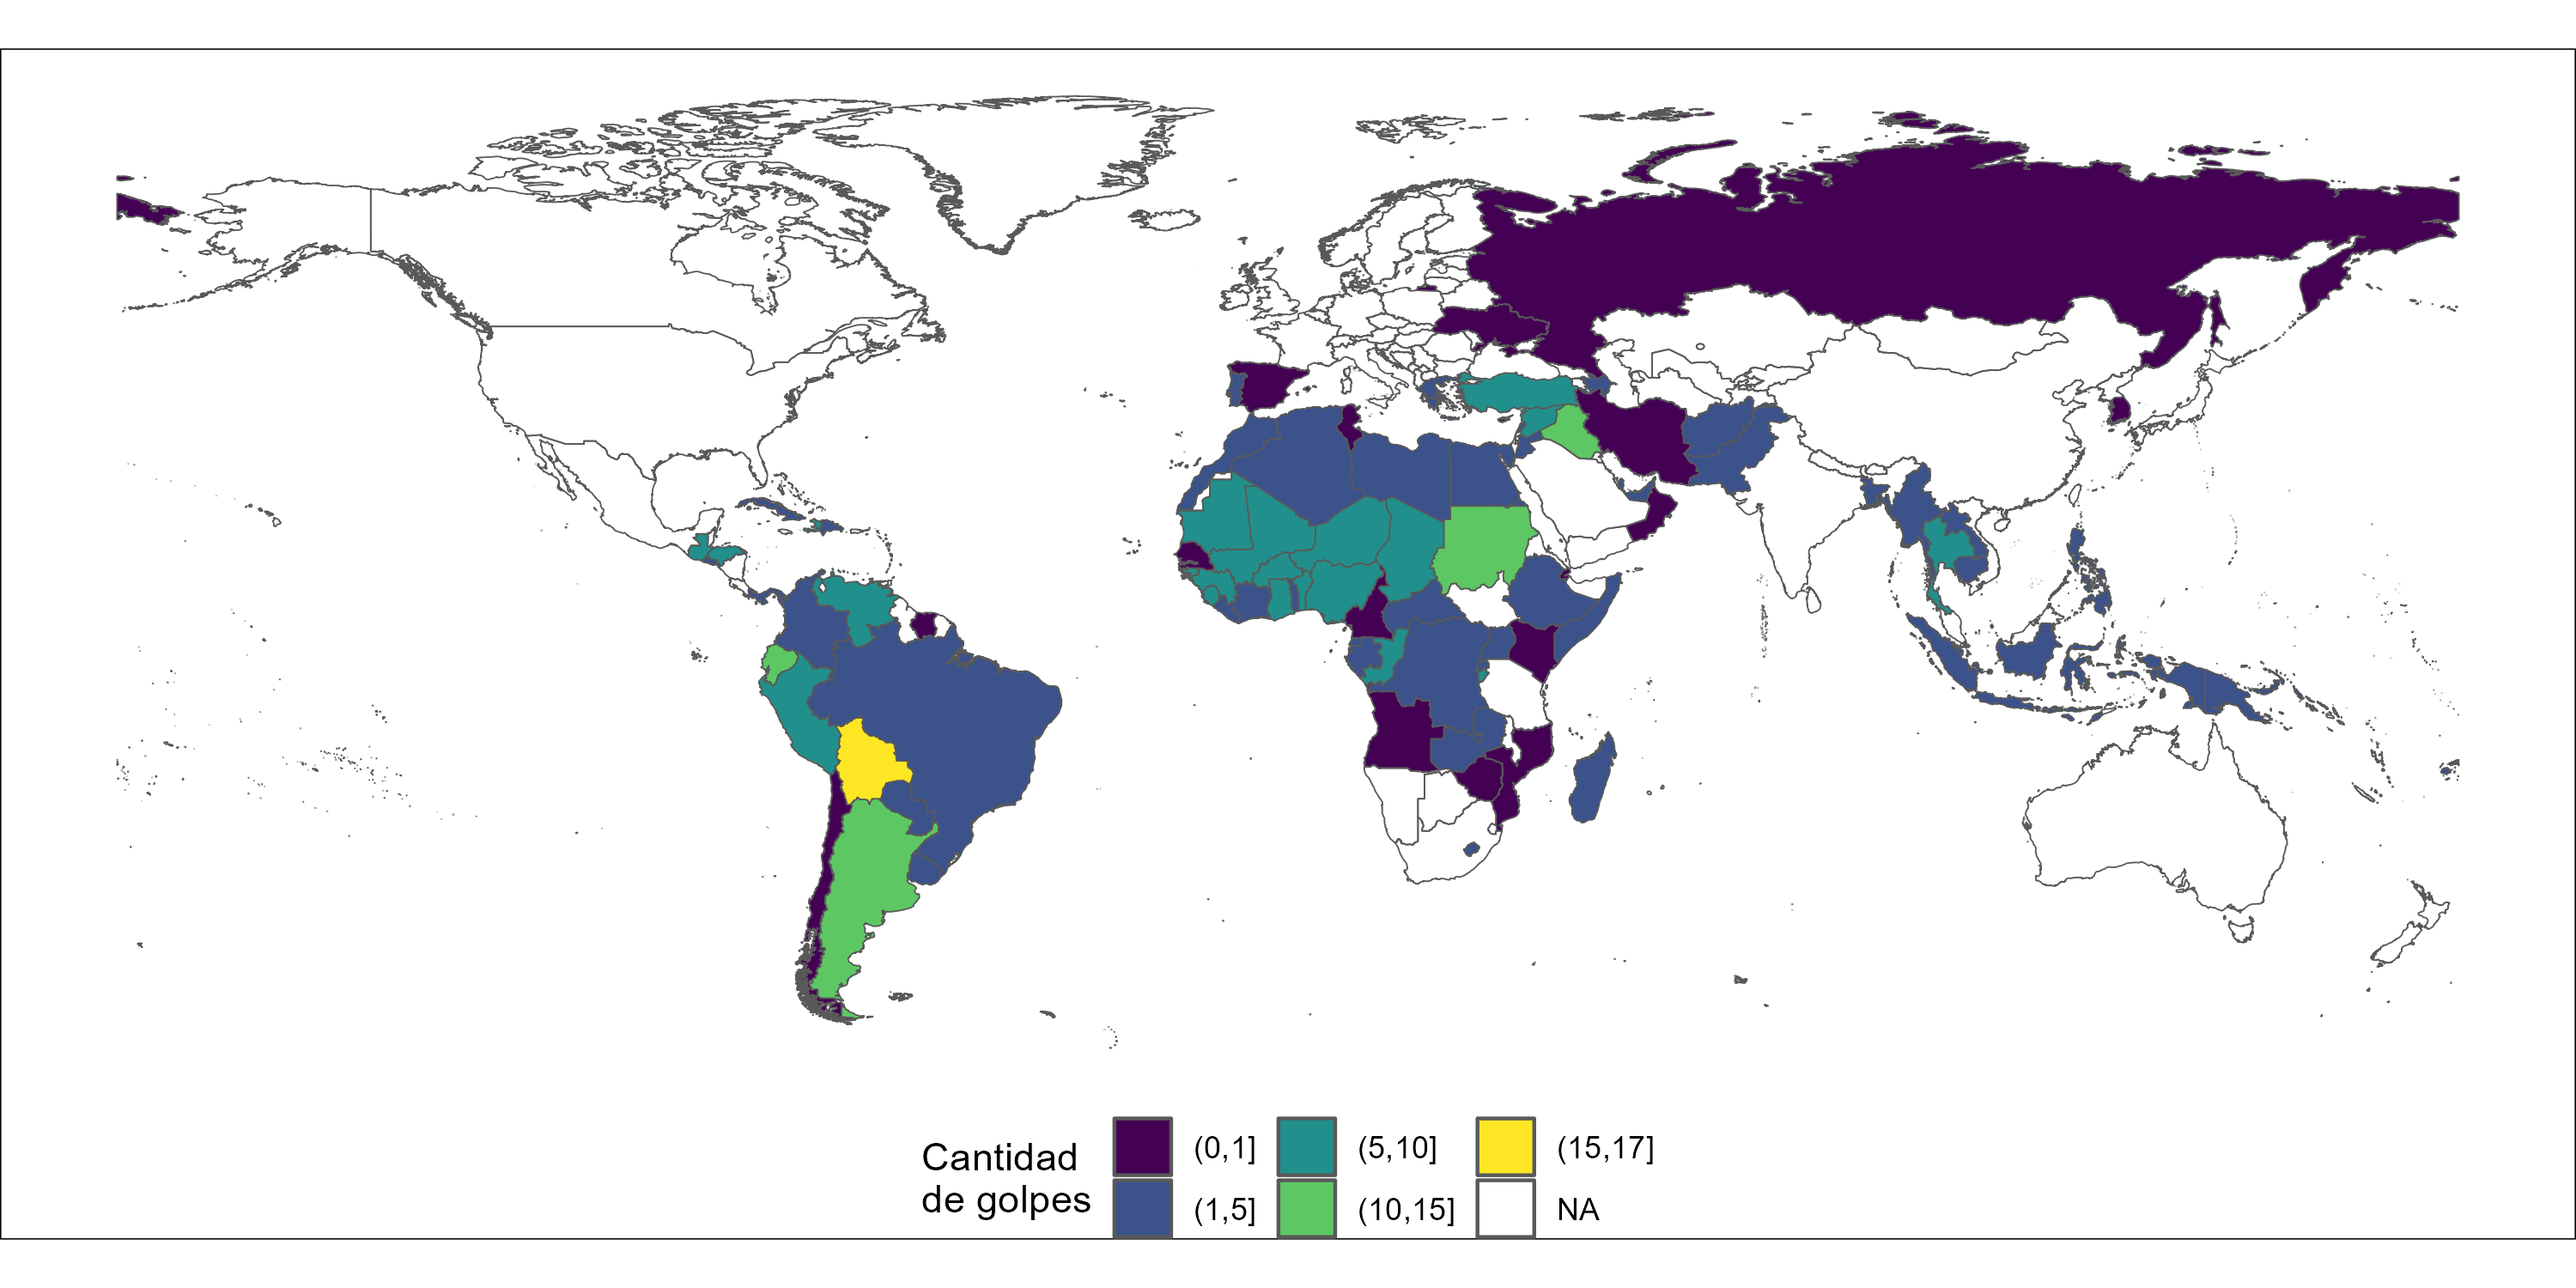
\includegraphics[width=1\textwidth]{2_golpes.png}
 \caption{Golpes de estado período (1950-2023) Fuente: \cite{Pow11} \label{fig::mapa_golpes}}
\end{figure}

Con mayor precisión, observamos que la región del Sahel se destaca con respecto a sus
vecinos africanos. Los países en donde más golpes de estado se han producido son
Bolivia (17), Sudán (14), Argentina (13), Ecuador (11), Iraq (11), Siria (11), 
Guatemala (10) y Tailandia (10).

Desagregando por década se observan algunos cambios, así como la persistencia en 
algunas regiones. La región del Sahel y varias naciones circundantes fueron 
persistentemente afectadas por golpes de estado desde los años 60. En América del 
Sur, en cambio, la presencia casi total de situaciones golpistas en la región se 
fue acotando a partir de los años 80 hasta finalmente desaparecer en el siglo 
xxi. Para observar con más detalle y discriminado por años y países se puede ver 
la figura \ref{fig:golpes_anios}.

\begin{figure}[H]
 \centering 
 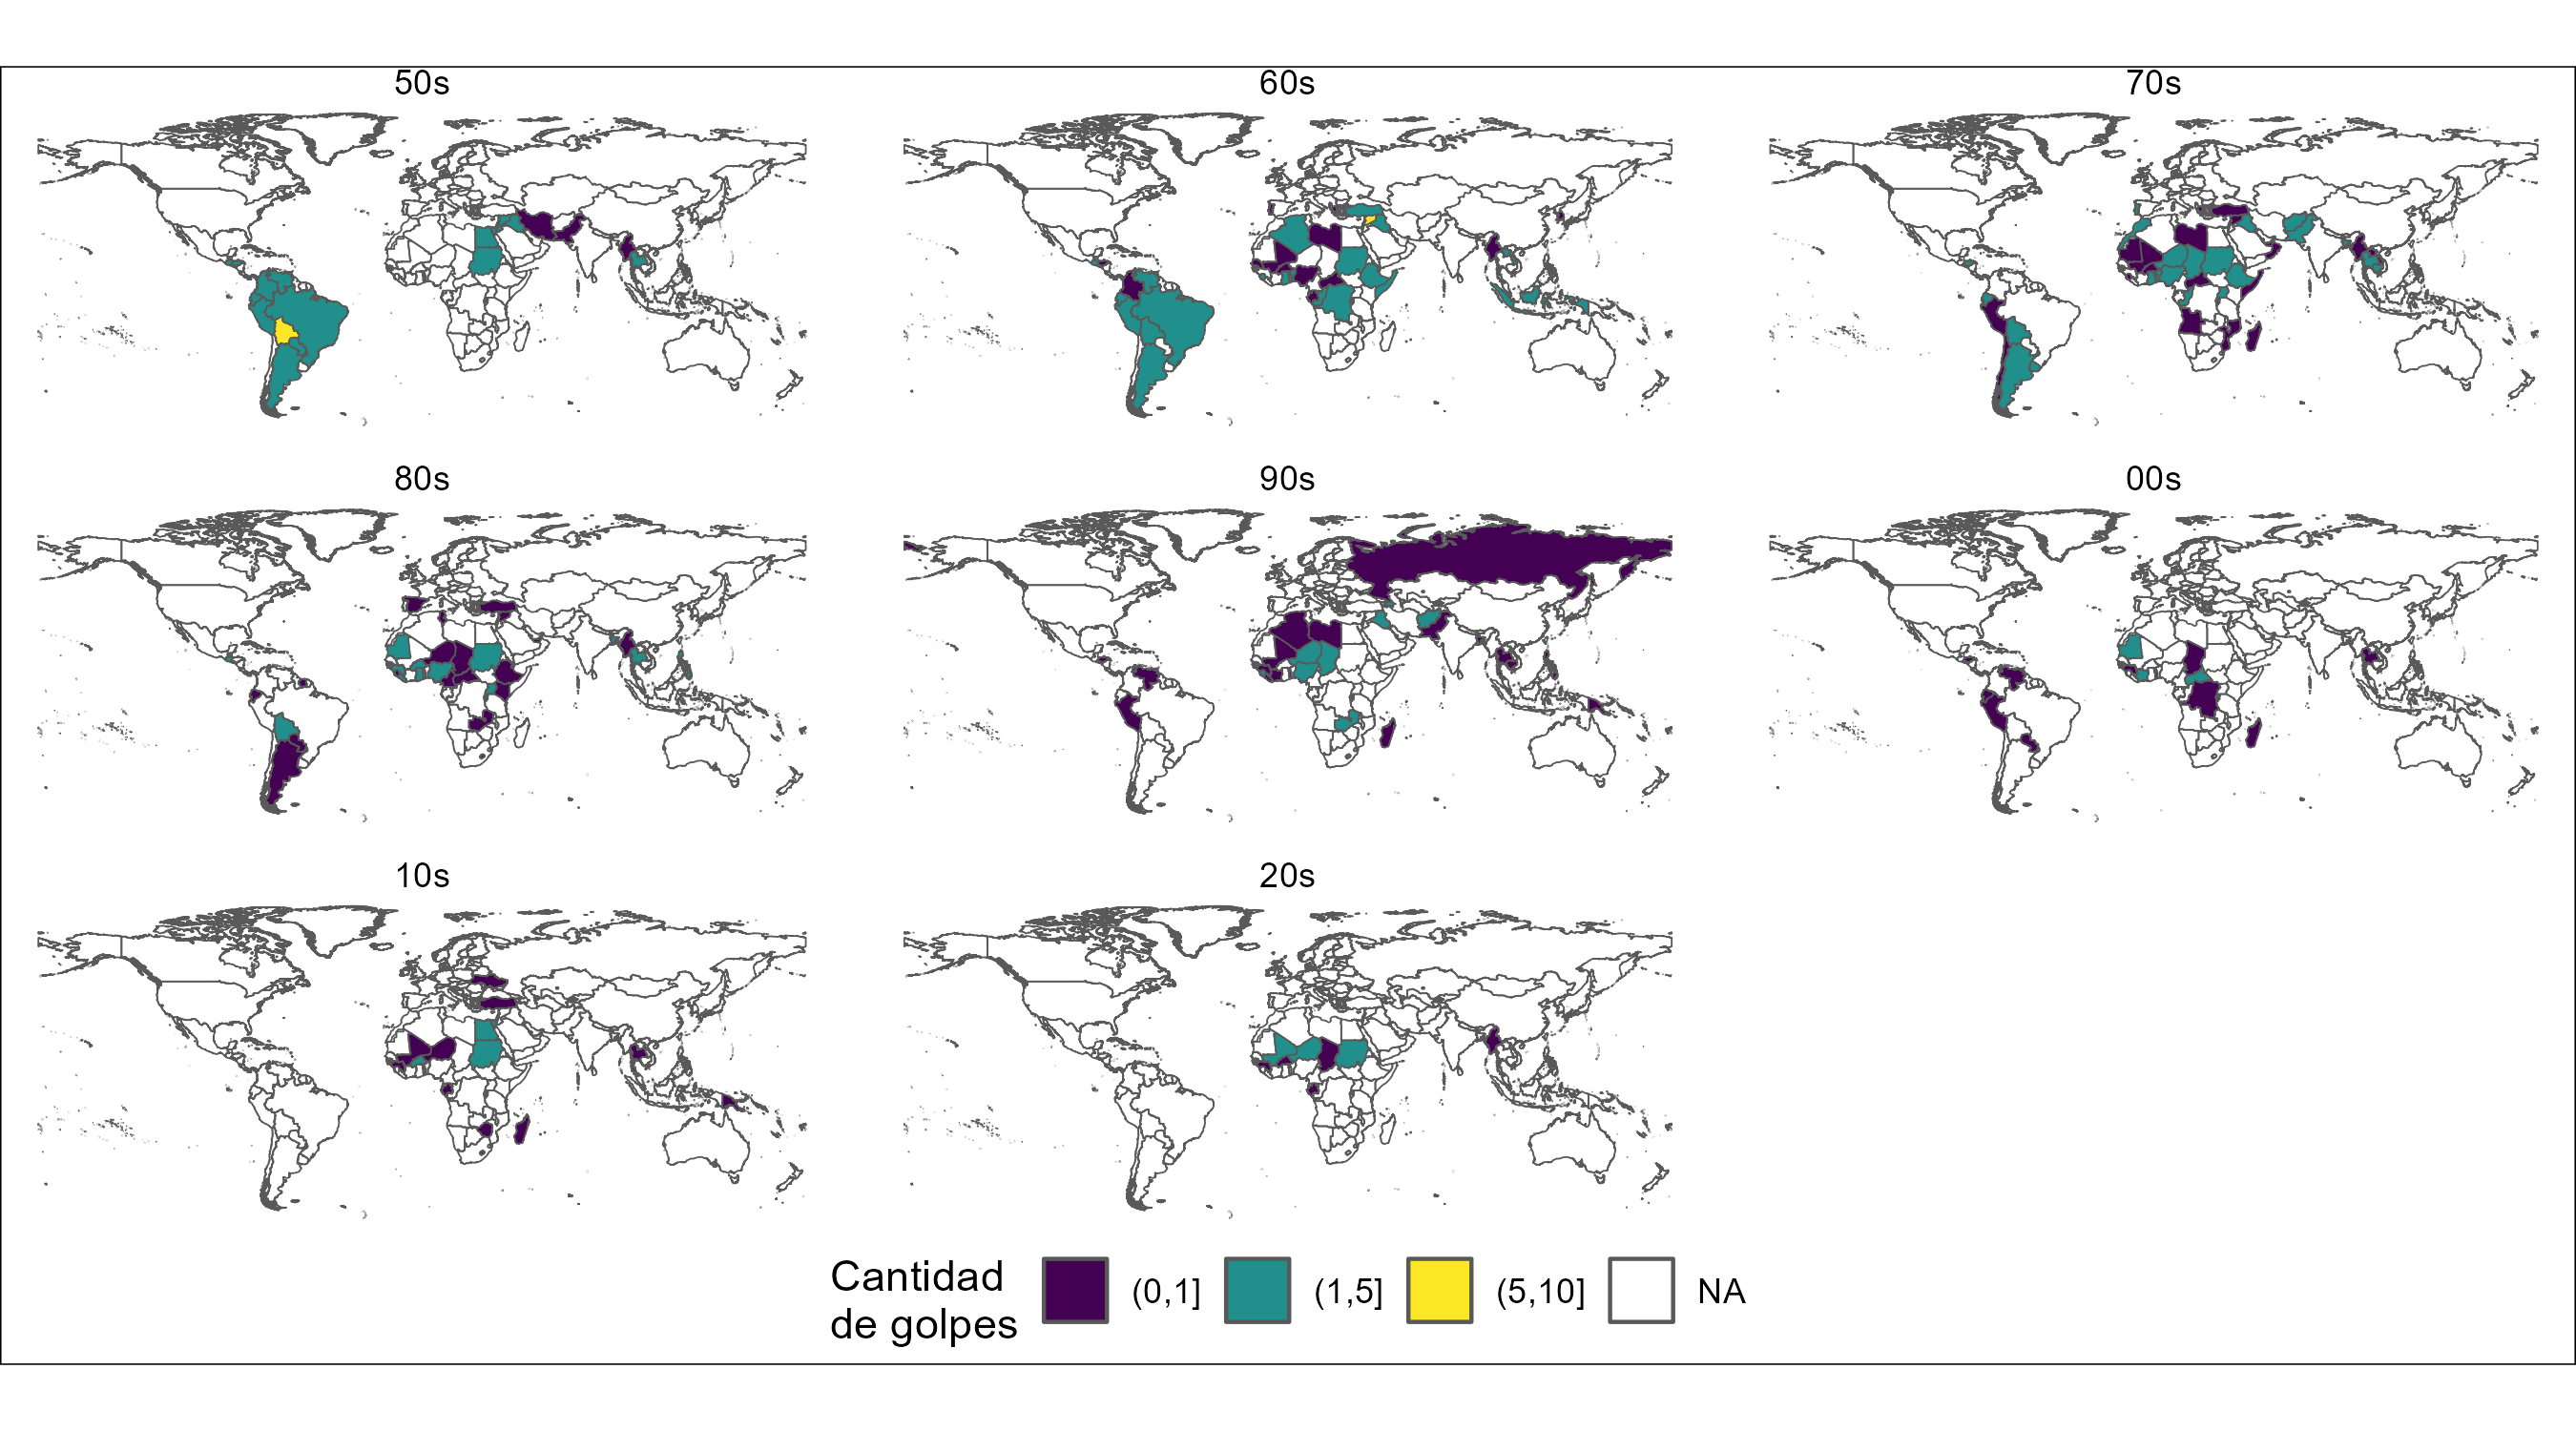
\includegraphics[width=1\textwidth]{3_golpes_decadas.png}
 \caption{Conteo de golpes por década Fuente:\cite{Pow11} \label{fig:golpes_decadas}}
\end{figure}

\section{Resultados y discusión}

\subsection{Performance de los modelos}
En primer lugar, se realizó la optimización bayesiana de ambos modelos según lo indicado
en la metodología. En el caso de XGBoost se pudo realizar las 100 iteraciones sin mayores
inconvenientes, tomando los valores óptimos de hiperparámetros para el entrenamiento 
final. Con respecto a Random Forest, en cambio, se alcanzaron 44 iteraciones, debido a que cada
iteración consumía una gran cantidad de tiempo (en promedio una hora) y no se observaban
mejoras significativas en el AUC. De las iteraciones generadas, se tomaron los hiperparámetros
que daban mejor resultado y tardaban menos minutos en entrenar el modelo.

Una vez seleccionado los mejores hiperparámetros, se procede a entrenar los modelos en el
conjunto de entrenamiento final, el cual abarca los registros desde 1970 hasta 2019; así
como a evaluar el desempeño del mismo en los años 2020, 2021 y 2022 para emular el trabajo
realizado por el FMI.

Es importante destacar que existen dos enfoques para evaluar el modelo en los años de
testeo: por un lado se pueden evaluar todos los años en su conjunto utilizando como datos
de entrenamiento los registros hasta el año anterior del primer año de validación. Una
opción alternativa es ir entrenando el modelo hasta el año anterior al de validación para
cada año individualmente, de manera de poder utilizar todos los años anteriores y no 
perder performance. Para este trabajo utilizamos el primer enfoque, es decir que entrenamos los 
modelos hasta 2019 y los evaluamos en todos los años de evaluación a la vez, de manera de
aprehender de manera general la importancia de cada variable en la predicción de la
variable objetivo.

En el cuadro \ref{tab:performance} observamos el desempeño de los modelos en los años
de testeo. Por un lado, figura el AUC individual de cada año por separado, y por el otro
observamos el AUC acumulada, es decir evaluando en ese año junto con los anteriores.

\begin{table}[H]
 \centering
  \begin{tabular}{lcccc}
   \toprule
   & \multicolumn{2}{c}{XGBoost} & \multicolumn{2}{c}{Random Forest} \\
   Año & AUC   & AUC   & AUC   & AUC \\
      &     & acumulada&     & acumulada \\
   \midrule
   2020 & 1.000 & 1.000 & 1.000 & 1.000 \\
   2021 & 0.750 & 0.786 & 0.747 & 0.784 \\
   2022 & 0.667 & 0.750 & 0.667 & 0.749 \\
   \bottomrule
  \end{tabular}
 \caption{Área bajo la curva ROC por año puntual y acumulado (XGBoost y 
 Random Forest) \label{tab:performance}}
\end{table}

Lo primero que podemos observar es que ambos modelos logran una performance perfecta 
para el año 2020, lo cual resulta esperable ya que cuentan con información del año 
inmediatamente anterior y a que sólo deben predecir un golpe de estado (en Mali).
Adicionalmente, la performance decae en los años siguientes, 
lo cual impacta en el valor del AUC acumulada. Comparando ambos modelos, observamos
que XGBoost fue ligeramente superior en el año 2021 con respecto a Random Forest.
Como no es una diferencia significativa, vamos a analizar ambos modelos para observar
si utilizan diferentes variables para sus predicciones.

Puesto que los casos positivos son apenas diez, aprovecharemos para visualizar la performance
de los modelos en cada uno de los casos. Adicionalmente, incorporamos el único falso positivo
predicho por Random Forest (Afganistán en el año 2021). La lista figura en el cuadro 
(Cuadro \ref{tab:resultados}).

\begin{table}[H]
 \centering
  \begin{tabular}{lrlll}
   \toprule
   país & año & ¿Hubo golpe? & Random Forest & XGBoost \\
   \midrule
   Malí & 2020 & Sí & Verdadero positivo & Verdadero positivo \\
   Birmania/Myanmar & 2021 & Sí & Verdadero positivo & Verdadero positivo \\
   Malí & 2021 & Sí & Falso negativo & Falso negativo \\
   Sudán & 2021 & Sí & Verdadero positivo & Verdadero positivo \\
   Afganistán & 2021 & No & Falso positivo & Verdadero negativo \\
   Níger & 2021 & Sí & Falso negativo & Falso negativo \\
   Guinea & 2021 & Sí & Verdadero positivo & Verdadero positivo \\
   Chad & 2021 & Sí & Falso negativo & Falso negativo \\
   Burkina Faso & 2022 & Sí & Verdadero positivo & Verdadero positivo \\
   Guinea-Bisáu & 2022 & Sí & Falso negativo & Falso negativo \\
   Santo Tomé y Príncipe & 2022 & Sí & Falso negativo & Falso negativo \\
   \bottomrule
  \end{tabular}
 \caption{Falsos negativos y verdaderos positivos (Random Forest) \label{tab:resultados}}
\end{table}

Ambos modelos predicen correctamente el único golpe del año 2020 en Mali. A su
vez, fallan en predecir los golpes de Mali, Níger y Chad de 2021; así como fallan en predecir
casi todos los golpes del 2022, a excepción del de Burkina Faso. La única discrepancia entre
los algoritmos surgió con respecto a Afganistán en el año 2021: fue el único caso de falso
positivo predicho por Random Forest, mientras que XGBoost logró categorizarlo correctamente
como negativo.

Profundizando en el análisis de la performance, vamos a observar la probabilidad asignada
a cada caso por el algoritmo. Mirando la probabilidad de Random Forest 
(figura \ref{fig:prob_rf}), llama la atención como el caso de Afganistán en 2021 figura
en los primeros puestos de la lista, superando incluso a cuatro casos positivos ¿Por qué sucedió esto?
Resulta útil remitirnos nuevamente a la definición de golpes de Estado de Powell y Thyne:
\textit{intentos ilegales y manifiestos por parte de las fuerzas armadas u de otras elites dentro
del aparato estatal de derrocar al gobierno en ejercicio} (\cite[p.~252]{Pow11}). En el caso de 
Afganistán, la toma del poder no fue perpetrada por sectores internos del Estado afgano, sino
por un ejército externo (en este caso, el movimiento Talibán).

\begin{figure}[H]
 \centering 
 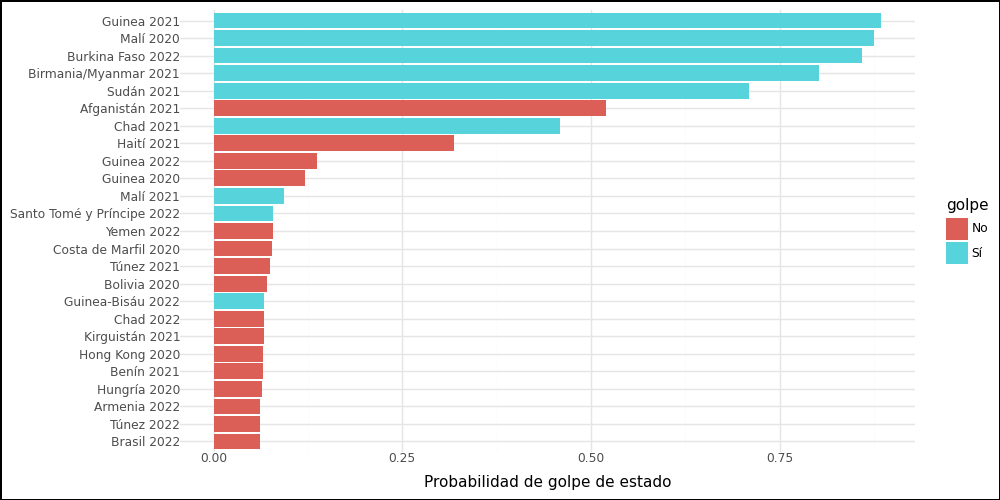
\includegraphics[width=1\textwidth]{5_prob_rf.png}
 \caption{Predicción probabilística años 2020-2022 (Random Forest) \label{fig:prob_rf}}
\end{figure}

En cambio, Xgboost separa más consistentemente los casos positivos de los negativos
en su asignación de probabilidades (figura \ref{fig:prob_xgb}). Incluso posiciona en sexto lugar
a Chad en 2021, si bien no lo predice como positivo. De todas formas, en ambos casos 
Sao Tome y Príncipe en 2022 así como Guinea-Bissau en 2022 figuran bastante abajo en el ranking
lo cual hace esperable que fallen en lograr predecir sus respectivos golpes de Estado. Por 
último, existe un único caso positivo que ni siquiera alcanzó las primeras 25 posiciones: nos
referimos a Níger en 2021. Random Forest le asignó una probabilidad del 4,46 por ciento, 
posicionándolo en el puesto 36. Aún más interesante, XGBoost le asignó apenas una probabilidad
de 0,033 por ciento (puesto 44). Profundizando en este caso, descubrimos que lo que sucedió tanto en 
Níger como en Guinea-Bisáu y Santo Tomé y Príncipe fueron intentos fallidos de golpe de Estado.
Esto nos puede dar una pista de qué tan efectivos son estos modelos para predecir golpes de Estado 
que no llegan a concretarse.

\begin{figure}[H]
 \centering 
 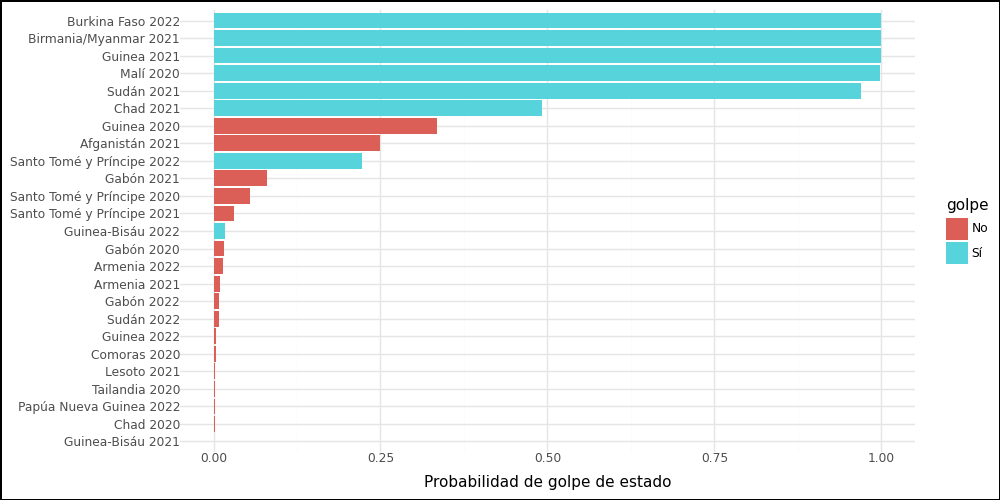
\includegraphics[width=1\textwidth]{6_prob_xgb.png}
 \caption{Predicción probabilística años 2020-2022 (XGBoost) \label{fig:prob_xgb}}
\end{figure}

Con el objetivo de profundizar los motivos para predecir correcta o incorrectamente los casos
expuestos, así como para enriquecer el análisis sobre los factores explicativos del fenómeno 
estudiado, realizaremos un análisis de las variables más relevantes para la predicción de golpes
de acuerdo a los dos algoritmos. Utilizaremos la importancia de las variables, incluido dentro
de los modelos entrenados, así como enfoques externos con los valores Shapley.

\subsection{Análisis de variables}
A continuación, pasaremos a evaluar la relevancia de las distintas variables del dataset
para la predicción del modelo. De esa manera, podremos extraer elementos para determinar
o reforzar los posibles causales de un golpe de estado en un territorio determinado. En 
primer lugar, utilizaremos la importancia de las variables según Random Forest, la cual
se puede observar en la figura \ref{fig:feat_imp_rf}\footnote{Los nombres de las variables fueron
traducidas y resumidas del libro de códigos de la base de datos para una vista amigable.
Se puede verificar el nombre codificado y original de las variables en el cuadro \ref{tab:vars}}.

En el caso de Random Forest la importancia de las variables indica cuánto disminuye la impureza
de los nodos (en este caso, medida con el índice de Gini, establecido por default en el modelo de 
Scikit-Learn) al utilizar una variable para dividir los datos de un árbol de decisión, de los cuales
se obtiene un promedio para todo el ensamble de árboles.

Las barras indican el porcentaje de importancia de las 10 variables con mayor peso. En total, estas 
diez variables representan alrededor del 75 por ciento de la importancia. En general, todas las 
variables están relacionadas con la forma de gobierno, con la influencia de las fuerzas armadas en el 
mismo o con la misma variable objetivo en años anteriores. Entre el primer y el cuarto lugar figuran 
variables que reflejan muy evidentemente una relación con la presencia de golpes de estado, como 
tener la legislatura cerrada o abortada o que el ejecutivo no sea más electo.

\begin{figure}[H]
 \centering 
 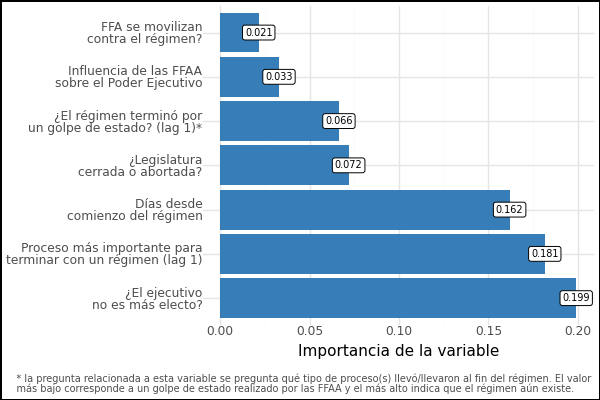
\includegraphics[width=1\textwidth]{7_feature_importance_rf.png}
 \caption{Importancia de las variables para predicción 2020-2022 (Random Forest) \label{fig:feat_imp_rf}}
\end{figure}

\begin{figure}[H]
 \centering 
 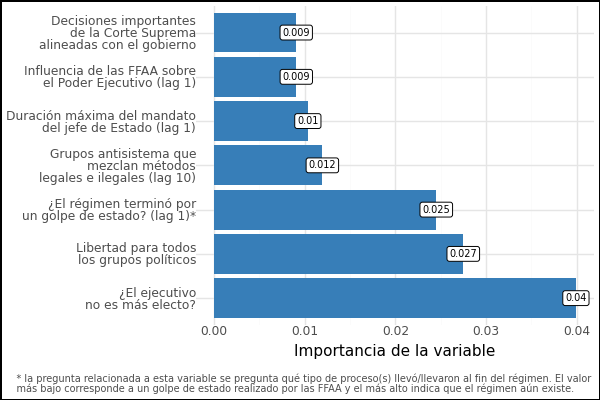
\includegraphics[width=1\textwidth]{8_feature_importance_xgb.png}
 \caption{Importancia de las variables para predicción 2020-2022 (XGBoost) \label{fig:feat_imp_xgb}}
\end{figure}

Ahora observaremos una variable similar para XGBoost en la figura \ref{fig:feat_imp_xgb}, aunque la 
importancia de la variable para este algoritmo significa cuántas veces aparece cada variable
en cualquier nodo de decisión de los árboles del modelo, normalizado por la cantidad de veces
que se realizaron divisiones en todos los árboles. Si bien se encuentran similitudes con Random Forest,
XGBoost destaca otras variables que llaman la atención, como la libertad de grupos sociales, las 
decisiones de la Corte Suprema que puedan ser adversas al gobierno, la duración del mandato del jefe de 
Estado y los métodos de lucha de los grupos antisistema presentes en el país.

Una desventaja de esta métrica es que no permite evaluar el uso de estos atributos comparado con el valor
de los mismos. Es por eso que incorporamos un análisis utilizando valores Shapley Values. En el eje Y 
figuran las primeras 11 variables con mayor valor de Shapley y en el eje X figura el valor Shapley, 
visualizando la distribución de los casos en forma de violín y los valores atípicos como puntos. Finalmente, 
el color de los violines y de los puntos indica el valor de la variable en cuestión.

\begin{figure}[H]
 \centering
 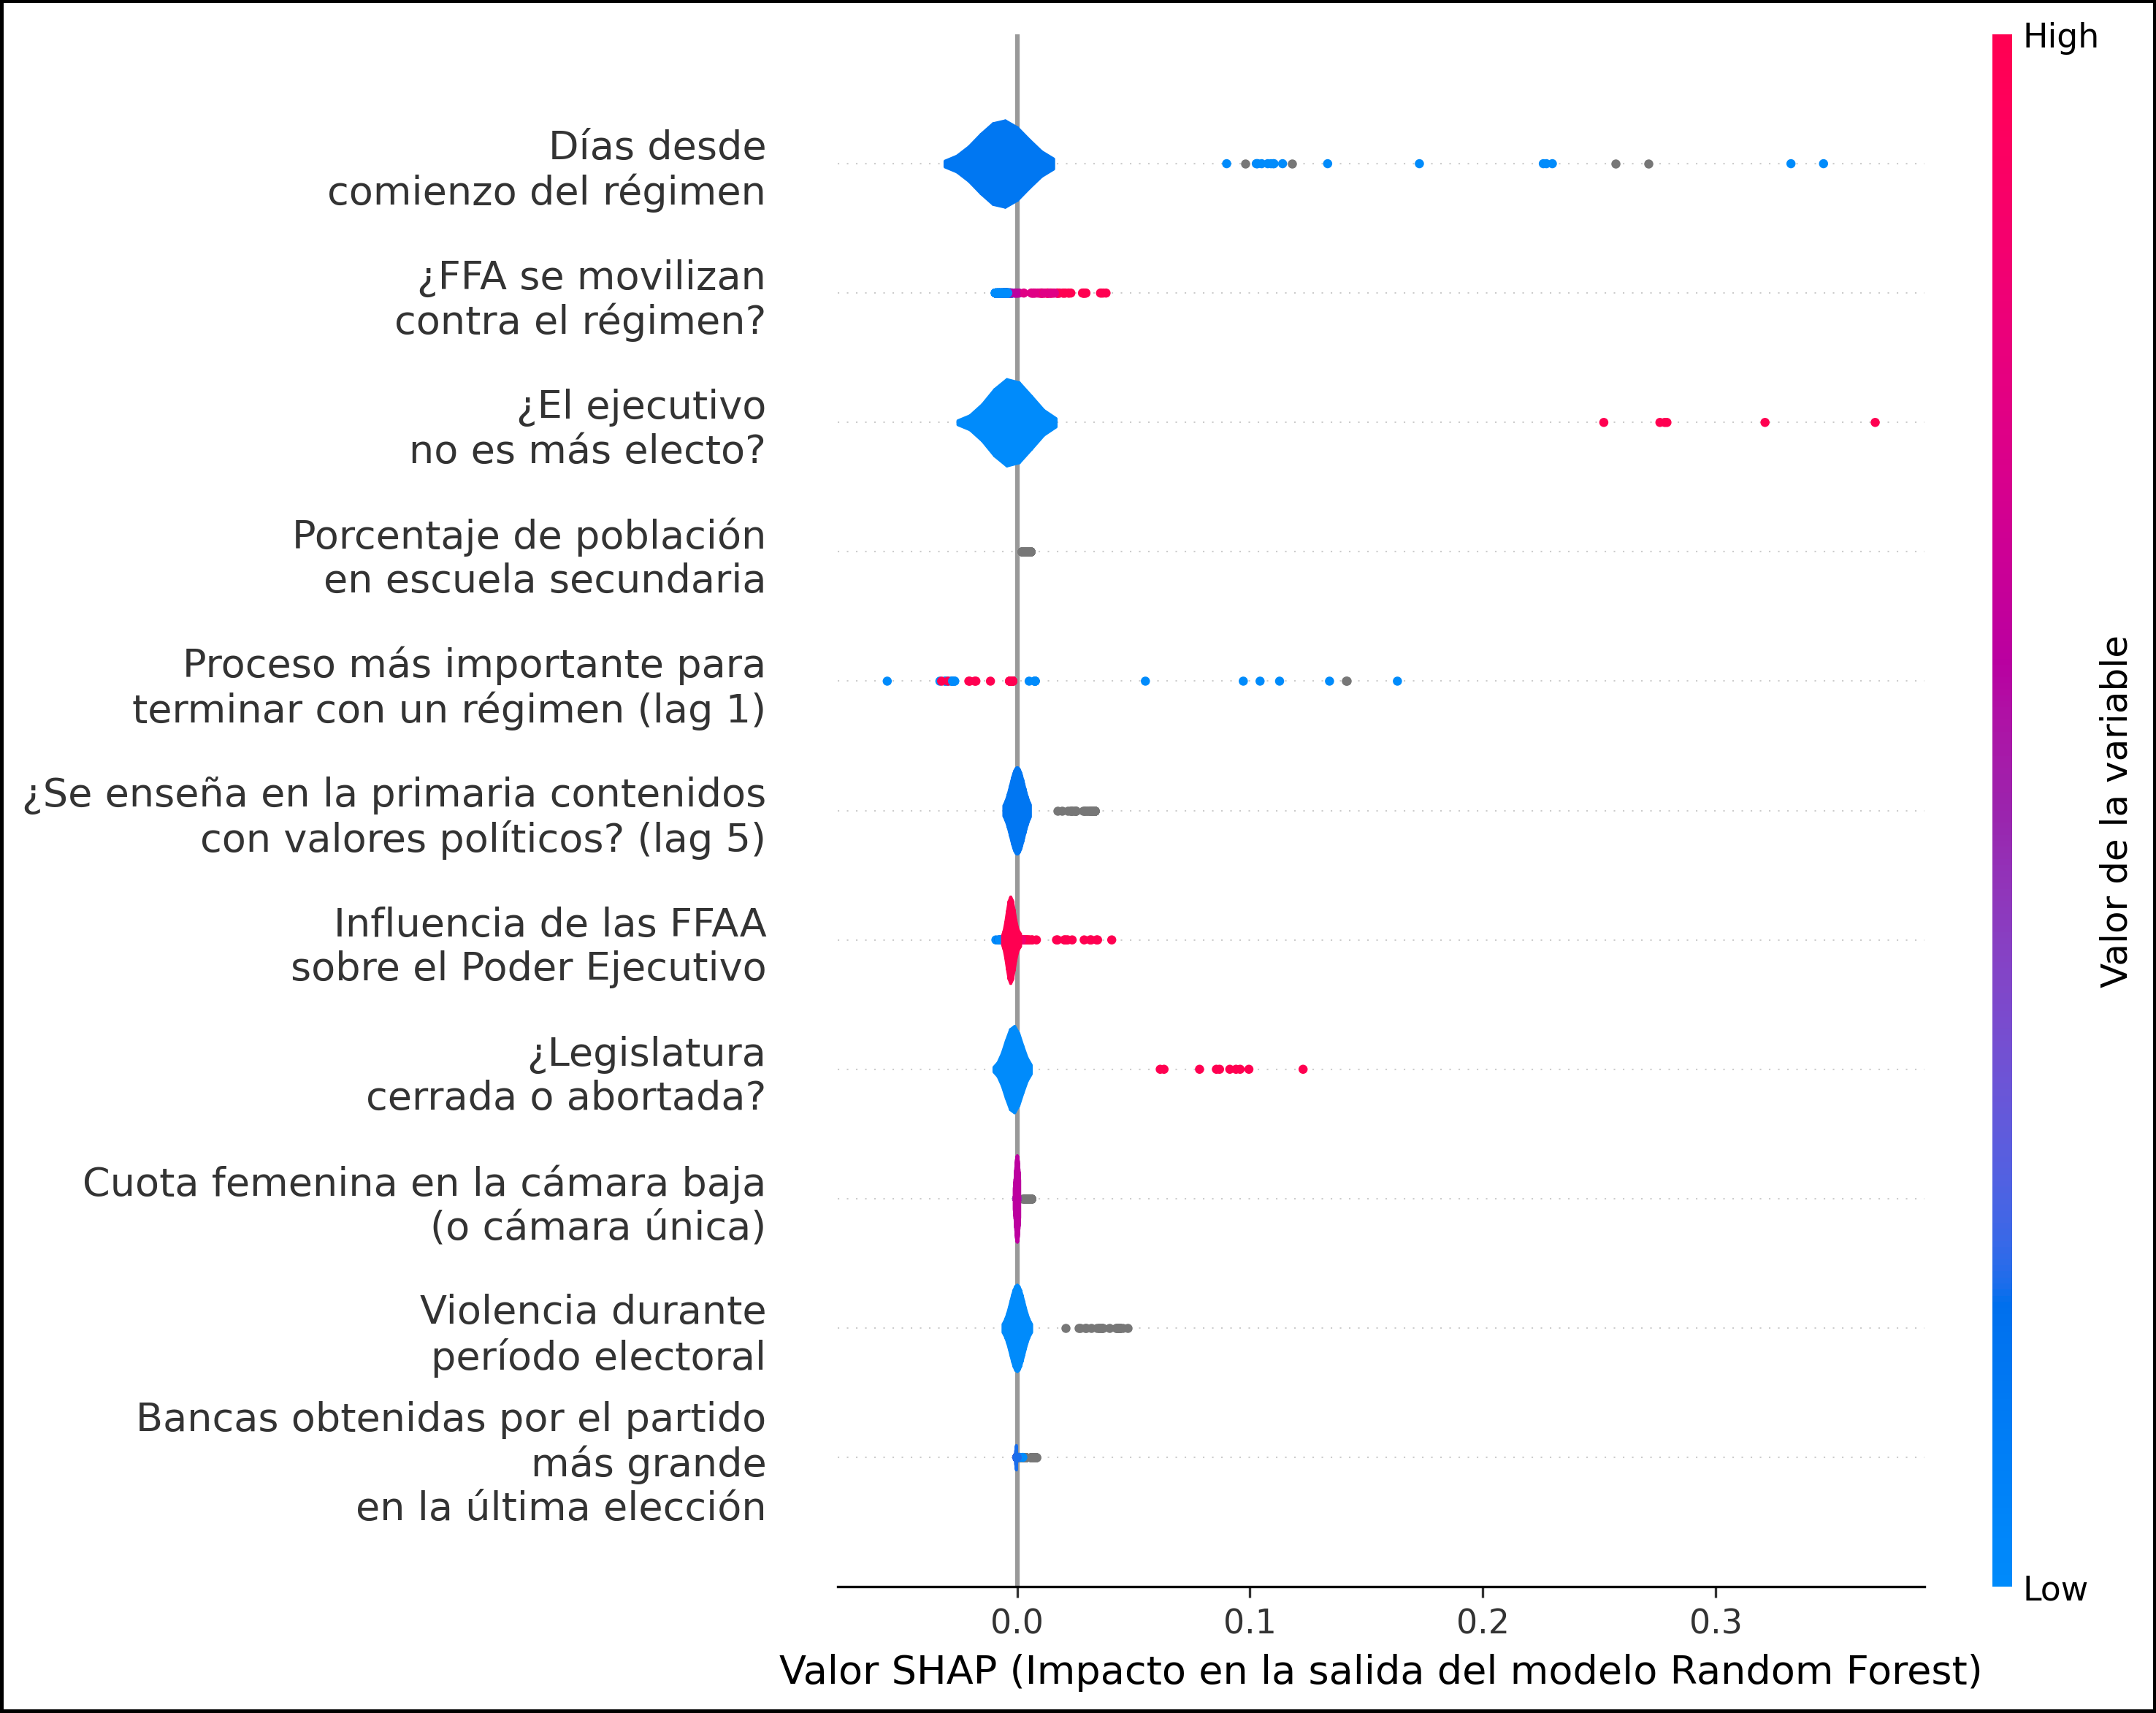
\includegraphics[width=1\textwidth]{9_shapley_values_rf.png}
 \caption{Shapley values para predicción 2020-2022 (Random Forest)\label{fig:shapley_rf}}
\end{figure}

Si bien en la figura \ref{fig:shapley_rf} algunas variables figuran también en el gráfico de la 
importancia de las variables, podemos destacar algunas diferencias. Primero, figura la enseñanza de 
valores políticos en la escuela, en cuyos valores nulos tienen alto valor Shapley. Lo mismo sucede
con la violencia durante un período electoral.

Adicionalmente, si bien la cantidad de días del régimen también figura en el gráfico de la 
importancias de las variables, esta visualización permite observar también cómo influye el valor
de la variable en sus valores Shapley. Allí se observa que los casos con menor valor en la variable 
(es decir, con menores días del régimen) tienen mayor valor Shapley e inclina la balanza hacia la 
predicción de un caso positivo. Se puede inferir de esto último que un régimen joven es más 
inestable y, por lo tanto, propensa a sufrir un nuevo cambio de régimen mediante un golpe.

Para profundizar el análisis vamos a observar los casos positivos y falsos negativos para
saber qué valores obtuvieron en las variables más destacadas de la figura \ref{fig:shapley_rf}.

\begin{table}[H]
 \centering

 \begin{tabular}{lrrrlll}
  \toprule
  país & año & v2regdur & shap & golpe & Random Forest & exitoso \\
  \midrule
  Sudán & 2021 & 0 & 0.346 & Sí & Verdadero positivo & Sí \\
  Birmania/Myanmar & 2021 & 0 & 0.332 & Sí & Verdadero positivo & Sí \\
  Guinea & 2021 & 0 & 0.230 & Sí & Verdadero positivo & Sí \\
  Burkina Faso & 2022 & 0 & 0.227 & Sí & Verdadero positivo & Sí \\
  Malí & 2020 & 0 & 0.226 & Sí & Verdadero positivo & Sí \\
  Afganistán & 2021 & 0 & 0.173 & No & Falso positivo & - \\
  Chad & 2021 & 0 & 0.090 & Sí & Falso negativo & No \\
  Santo Tomé y Príncipe & 2022 & 11230 & -0.006 & Sí & Falso negativo & No \\
  Níger & 2021 & 3556 & -0.007 & Sí & Falso negativo & No \\
  Guinea-Bisáu & 2022 & 2749 & -0.007 & Sí & Falso negativo & No \\
  Malí & 2021 & 136 & -0.008 & Sí & Falso negativo & Sí \\
  \bottomrule
  \end{tabular} 
 \caption{Días desde comienzo régimen vs valores SHAP (Random Forest) \label{tab:shap_rf_regdur}}
\end{table}

En el cuadro \ref{tab:shap_rf_regdur} observamos el valor de los días desde comienzo del régimen
(con el nombre original de la base de datos para ahorrar espacio), el valor Shapley asociado de la 
misma variable, la predicción que hizo Random Forest y, adicionalmente, si esos golpes de Estado 
fueron exitosos o no\footnote{Powell y Thyne (\citeyear{Pow11}) 
cuentan con una base que distingue entre golpes exitosos y fallidos, pero llega hasta el año 2010. Por
ese motivo, se recurrió a diversas fuentes para construir la variable para estos casos.}. 
Además, el cuadro está ordenado de manera descendente a partir de los valores Shapley. Lo primero que 
podemos notar es que, a excepción de Chad en 2021, el hecho de tener cero días de duración de un 
régimen influye en un valor Shapley muy alto, ubicándose entre los más altos de toda la serie si se 
observa la escala de la figura \ref{fig:shapley_rf}. Eso parece influir en el hecho de que Afganistán 
sea predicho falsamente como positivo; así como que la mayoría de los golpes de Estado fallidos estén 
al final de la lista con una incorrecta predicción como negativo.

Ahora observaremos la variable que registra si el ejecutivo no es más electo:

\begin{table}[H]
 \centering
 \begin{tabular}{lrrrlll}
  \toprule
  país & año & v2x\_hosinter & shap & golpe & Random Forest & exitoso \\
  \midrule
  Chad & 2021 & 1 & 0.321 & Sí & Falso negativo & No \\
  Guinea & 2021 & 1 & 0.279 & Sí & Verdadero positivo & Sí \\
  Burkina Faso & 2022 & 1 & 0.278 & Sí & Verdadero positivo & Sí \\
  Malí & 2020 & 1 & 0.276 & Sí & Verdadero positivo & Sí \\
  Afganistán & 2021 & 1 & 0.252 & No & Falso positivo & - \\
  Birmania/Myanmar & 2021 & 0 & -0.002 & Sí & Verdadero positivo & Sí \\
  Sudán & 2021 & 0 & -0.002 & Sí & Verdadero positivo & Sí \\
  Santo Tomé y Príncipe & 2022 & 0 & -0.003 & Sí & Falso negativo & No \\
  Malí & 2021 & 0 & -0.003 & Sí & Falso negativo & Sí \\
  Níger & 2021 & 0 & -0.003 & Sí & Falso negativo & No \\
  Guinea-Bisáu & 2022 & 0 & -0.003 & Sí & Falso negativo & No \\
  \bottomrule
  \end{tabular}
\caption{¿El ejecutivo no es más electo? vs valores SHAP (Random Forest) \label{tab:shap_rf_hosinter}}
\end{table}

En este caso (cuadro \ref{tab:shap_rf_hosinter}) la relación entre la predicción y el valor de la 
variable y el Shapley no es tan directa, puesto que Chad en 2021 cuenta con el valor Shapley más 
alto de la lista, pero es predicho como negativo. Para el resto, se repite el patrón de predecir 
como negativo a valores bajos del valor Shapley y como positivo a valores altos.

\begin{table}[H]
 \centering
 \begin{tabular}{lrrrlll}
  \toprule
  país & año & v2regendtype\_lag\_1 & shap & golpe & Random Forest & exitoso \\
  \midrule
  Birmania/Myanmar & 2021 & 0 & 0.163 & Sí & Verdadero positivo & Sí \\
  Sudán & 2021 & 0 & 0.134 & Sí & Verdadero positivo & Sí \\
  Guinea & 2021 & 0 & 0.113 & Sí & Verdadero positivo & Sí \\
  Malí & 2020 & 0 & 0.104 & Sí & Verdadero positivo & Sí \\
  Burkina Faso & 2022 & 0 & 0.097 & Sí & Verdadero positivo & Sí \\
  Afganistán & 2021 & 1 & 0.055 & No & Falso positivo & - \\
  Santo Tomé y Príncipe & 2022 & 13 & -0.002 & Sí & Falso negativo & No \\
  Níger & 2021 & 13 & -0.002 & Sí & Falso negativo & No \\
  Malí & 2021 & 13 & -0.003 & Sí & Falso negativo & Sí \\
  Guinea-Bisáu & 2022 & 13 & -0.021 & Sí & Falso negativo & No \\
  Chad & 2021 & 10 & -0.056 & Sí & Falso negativo & No \\
  \bottomrule
  \end{tabular}
\caption{Proceso más importante para terminar con un régimen (lag 1) vs valores 
     SHAP (Random Forest) \label{tab:shap_rf_regend}}
\end{table}

En el cuadro \ref{tab:shap_rf_regend}, en cambio, parece percibirse claramente la manera en la que 
el algoritmo separó casos positivos de negativos. Aquí, el caso discutido de Afganistán figura en la
frontera entre los casos positivos y negativos. En cambio, todos los casos cuyo valor fue diez o más
fueron asignados como negativos, incluso Chad en 2021 que figuraba como fuerte candidato a una 
predicción positiva en variables anteriores. Nuevamente, todos los casos fallidos de golpes fueron
enviados al fondo de la lista. Retomando el caso de Afganistán, resulta relevante ahondar qué releva
esta variable y cómo se codifican sus variables. Esta variable pregunta por el proceso más 
importante que el experto considera que lleva al fin de un régimen\cite{CopMet24}. Las respuestas que 
figuran en el cuadro se codifican de la siguiente manera: 0=Un golpe de estado militar, 1=Un golpe de 
estado llevado a cabo por otros grupos diferentes a los militares, 13: El régimen aún existe. Afganistán
figura con el valor 1, por lo que podemos inferir que los expertos de esta base de datos calificaron
el proceso político en este país como un golpe de Estado, discrepando así con el artículo de Powell y 
Thyne, quienes no detectan un golpe de estado ni en 2021 ni en el año anterior, el cual es evaluado
en esta variable (puesto que es lag 1).

\begin{table}[H]
 \centering
 \begin{tabular}{lrrrlll}
  \toprule
  país & año & v2xlg\_leginter & shap & golpe & Random Forest & exitoso \\
  \midrule
  Birmania/Myanmar & 2021 & 1 & 0.123 & Sí & Verdadero positivo & Sí \\
  Guinea & 2021 & 1 & 0.096 & Sí & Verdadero positivo & Sí \\
  Burkina Faso & 2022 & 1 & 0.094 & Sí & Verdadero positivo & Sí \\
  Malí & 2020 & 1 & 0.091 & Sí & Verdadero positivo & Sí \\
  Guinea-Bisáu & 2022 & 1 & 0.086 & Sí & Falso negativo & No \\
  Chad & 2021 & 1 & 0.063 & Sí & Falso negativo & No \\
  Afganistán & 2021 & 1 & 0.062 & No & Falso positivo & - \\
  Santo Tomé y Príncipe & 2022 & 0 & -0.001 & Sí & Falso negativo & No \\
  Níger & 2021 & 0 & -0.001 & Sí & Falso negativo & No \\
  Malí & 2021 & 0 & -0.002 & Sí & Falso negativo & Sí \\
  Sudán & 2021 & 0 & -0.002 & Sí & Verdadero positivo & Sí \\
  \bottomrule
  \end{tabular}
\caption{¿Legislatura cerrada o abortada? vs valores SHAP (Random Forest) \label{tab:shap_rf_leginter}}
\end{table}

Por último, en el cuadro \ref{tab:shap_rf_leginter} analizamos la variable que evalúa si la legislatura 
fue cerrada o abortada en el país. Esta variable parece no haber tenido tanto peso como las anteriores 
para la predicción, puesto que figura el caso de Sudán 2021 que tuvo el valor Shapley más bajo del 
cuadro pero de todas formas fue predicho correctamente como positivo. De todas formas, un valor Shapley
mayor a 0,90 parece garantizar que el caso sea predicho como positivo.

\begin{figure}[H]
 \centering
 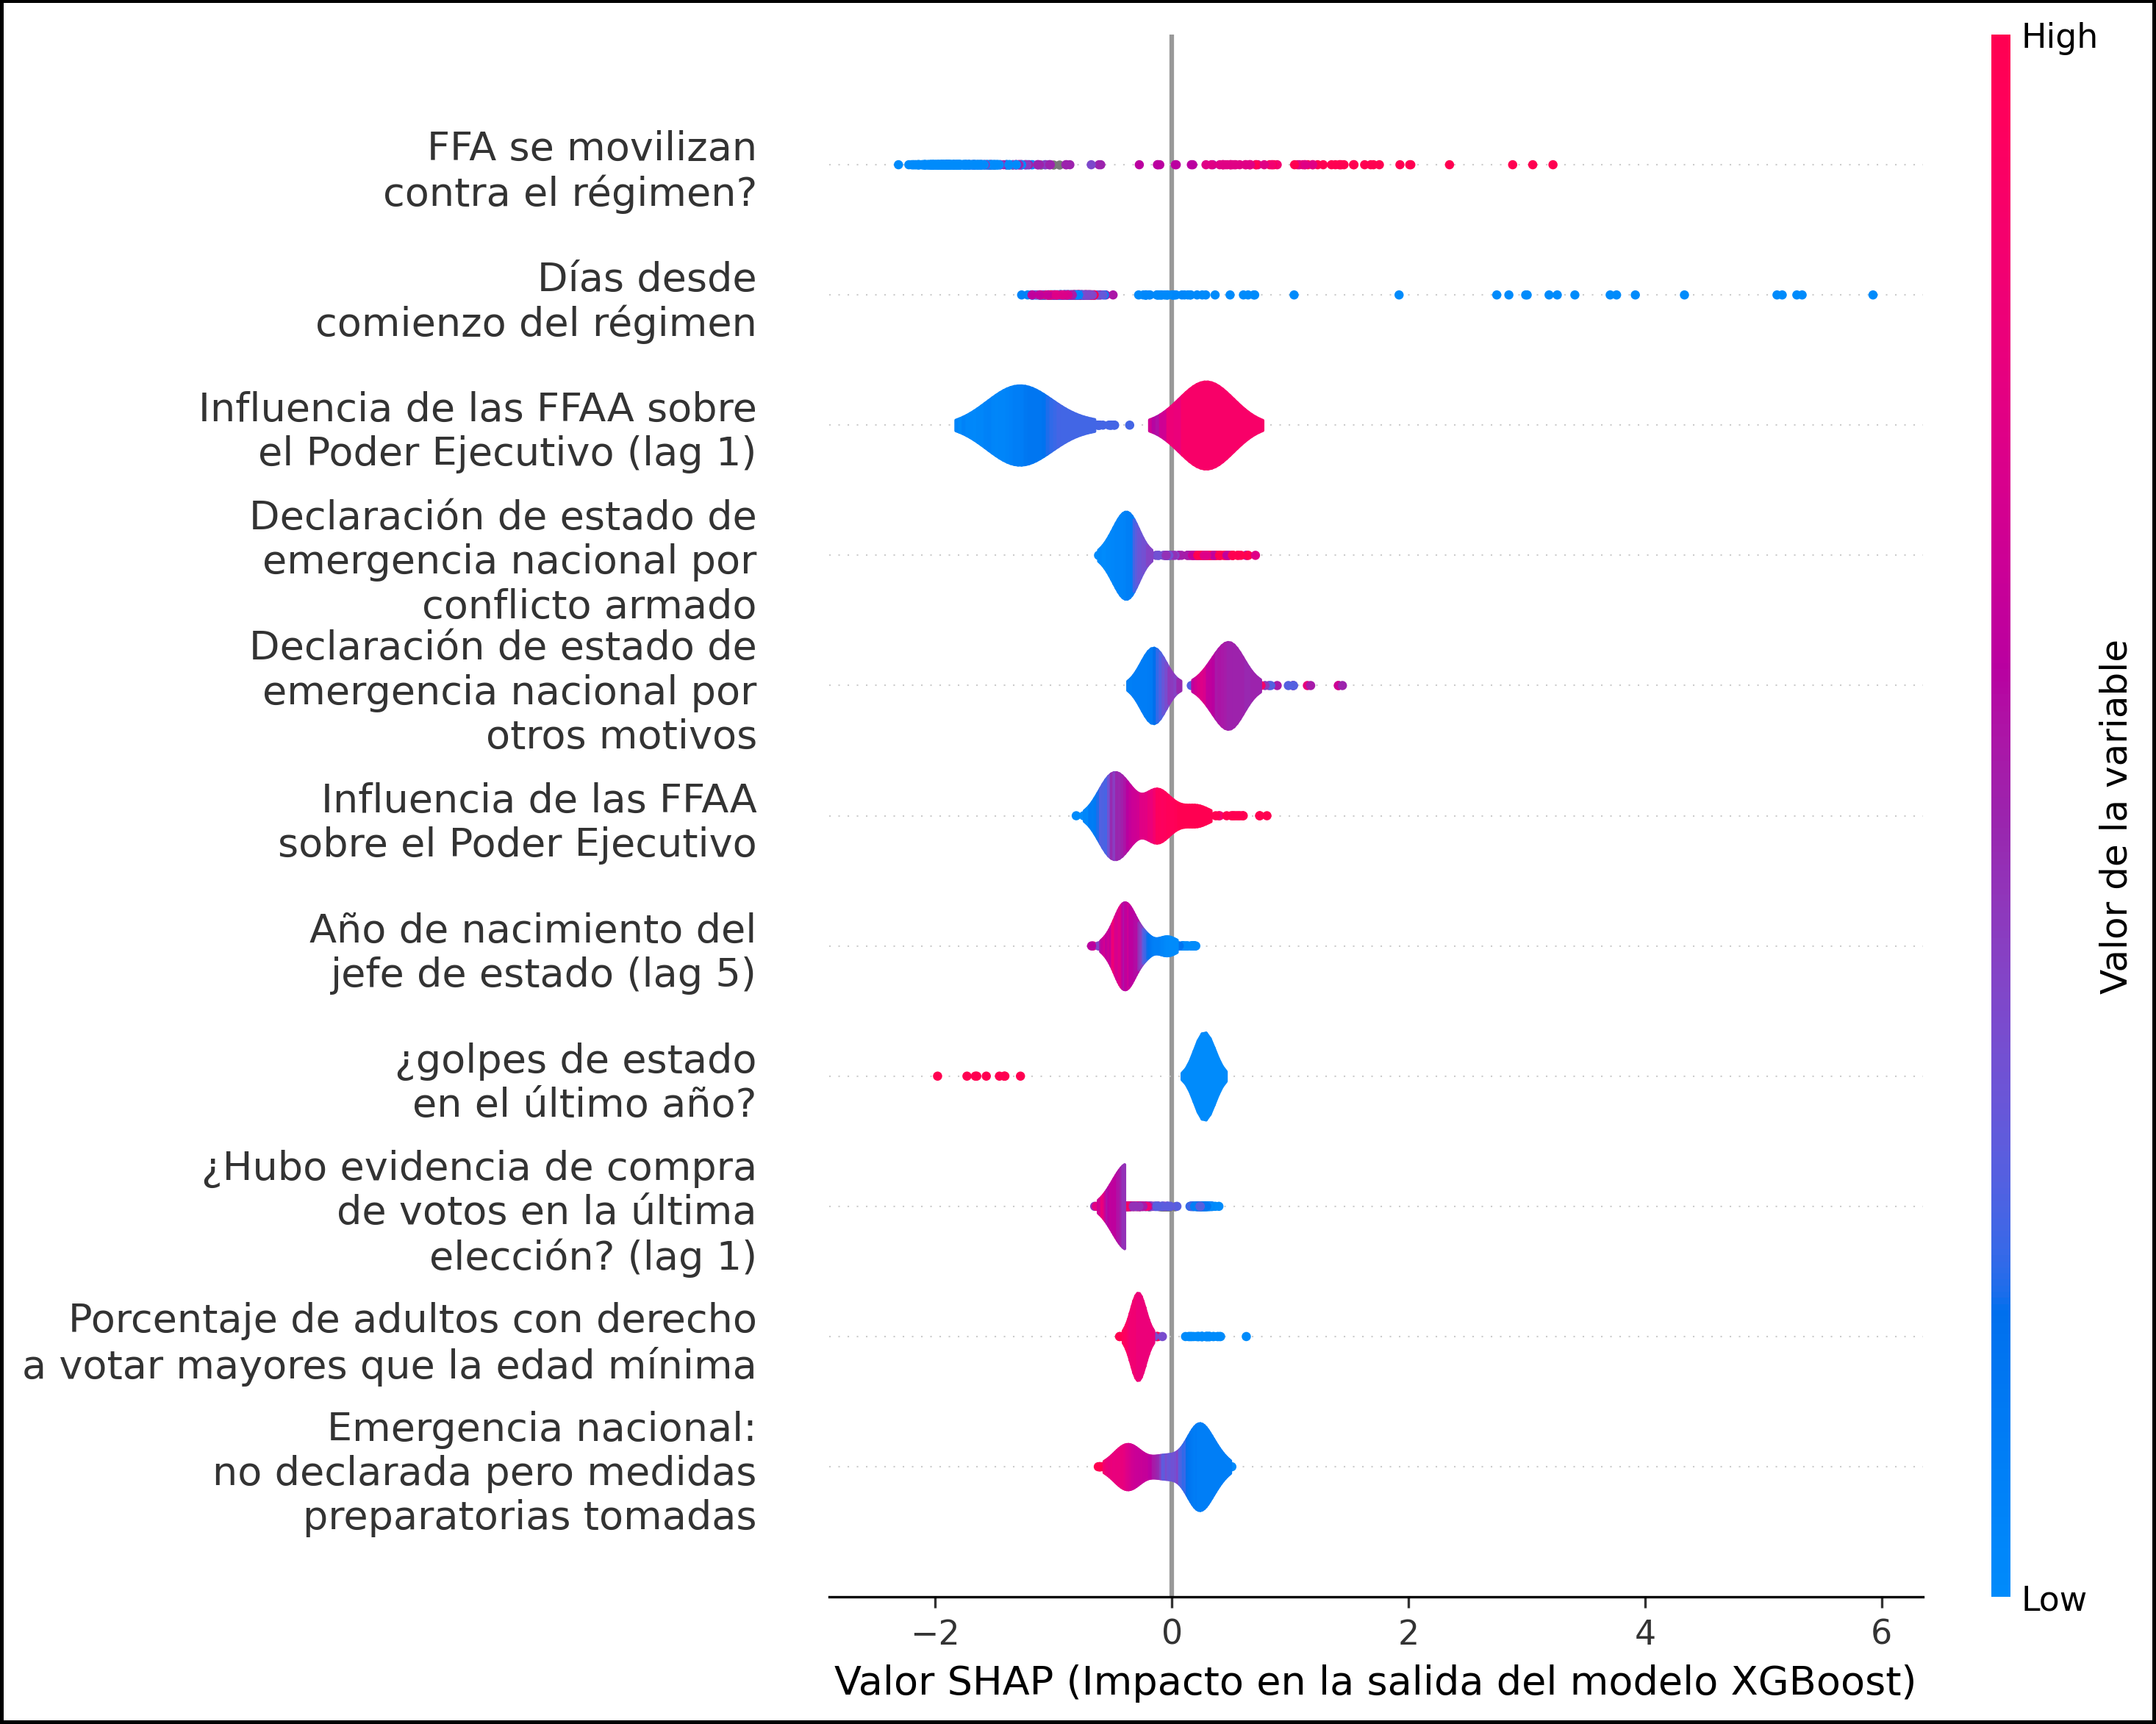
\includegraphics[width=1\textwidth]{10_shapley_values_xgb.png}
 \caption{Shapley values para predicción 2020-2022 (XGBoost)\label{fig:shapley_xgb}}
\end{figure}

Los valores Shapley de XGBoost (figura \ref{fig:shapley_xgb}) nos brinda nuevas perspectivas. 
Si bien comparte algunas variables con la visualización de Random Forest, figuran muchas más
casos con valores Shapley negativos, los cuales influyen para que el caso sea predicho como negativo. 
Así sucede con la influencia de las FFAA sobre el Poder Ejecutivo en el lag 1 (es decir, el año 
anterior al del registro), el cual si tiene un valor alto influye para que sea catalogado como 
positivo, mientras que si cuenta con valores bajos influye para el caso contrario.

Otros datos a destacar surgen de las variables que no figuran en Random Forest. En primer lugar,
figuran dos variables que evalúan la declaración de un Estado de emergencia en el país: ya sea si es 
por un conflicto armado o por otros motivos, tener un valor alto en estas variables inclina la balanza 
hacia tener un golpe de Estado. También el hecho de haber tenido un golpe de estado en el año anterior 
parece influir para que no suceda otro en el siguiente. Lo mismo sucede con la evidencia de compra de 
votos en el año anterior (lag 1) y en el porcentaje de adultos con derecho a votar mayores que la edad 
mínima. Nuevamente, observaremos los valores Shapley de las variables más relevantes de la figura
\ref{fig:shapley_xgb} para así observar con mayor detenimiento la manera en que el algoritmo tomó
sus decisiones.

Lo primero que se puede apreciar del cuadro \ref{tab:shap_xgb_regdur} es que asigna valores Shapley
muy similares a los que asignó Random Forest en el cuadro \ref{tab:shap_rf_regdur}. También envía casi
todos los golpes fallidos al fondo de la lista, fallando en su correcta predicción. Sin embargo,
XGBoost si fue exitoso en predecir que no sucedió un golpe de Estado en Afganistán, si bien parece
ubicarse en una posición similar al del cuadro \ref{tab:shap_rf_regdur}.

\begin{table}[H]
 \centering
 \begin{tabular}{lrrrlll}
  \toprule
  país & año & v2regdur & shap & golpe & xgboost & exitoso \\
  \midrule
  Birmania/Myanmar & 2021 & 0 & 5.927 & Sí & Verdadero positivo & Sí \\
  Sudán & 2021 & 0 & 5.328 & Sí & Verdadero positivo & Sí \\
  Malí & 2020 & 0 & 5.283 & Sí & Verdadero positivo & Sí \\
  Burkina Faso & 2022 & 0 & 5.159 & Sí & Verdadero positivo & Sí \\
  Guinea & 2021 & 0 & 5.115 & Sí & Verdadero positivo & Sí \\
  Afganistán & 2021 & 0 & 4.333 & No & Verdadero negativo & - \\
  Chad & 2021 & 0 & 2.747 & Sí & Falso negativo & No \\
  Malí & 2021 & 136 & 1.034 & Sí & Falso negativo & Sí \\
  Santo Tomé y Príncipe & 2022 & 11230 & -0.671 & Sí & Falso negativo & No \\
  Níger & 2021 & 3556 & -0.845 & Sí & Falso negativo & No \\
  Guinea-Bisáu & 2022 & 2749 & -0.883 & Sí & Falso negativo & No \\
  \bottomrule
  \end{tabular}
  \caption{Días desde comienzo régimen vs valores SHAP (XGBoost) \label{tab:shap_xgb_regdur}}
 \end{table}

Como último análisis de los valores Shapley en XGBoost observaremos dos variables significativas en
los cuadros \ref{tab:shap_xgb_regopp} y \ref{tab:shap_xgb_exmil}. En estos cuadros la separación entre
casos positivos y negativos no es tan lineal como en el caso anterior, sin embargo, se puede observar
que los valores altos de los valores Shapley en la movilización de las FFAA contra el poder ejecutivo
influyen para que el caso sea predicho como negativo. Interesantemente, aquí Afganistán figura como 
última en la lista, lo cual permite hipotetizar que esta variable ayuda a excluir a este país del grupo
de positivos.

 \begin{table}[H]
  \centering
  \begin{tabular}{lrrrlll}
   \toprule
   país & año & v2regoppgroupsact\_5 & shap & golpe & xgboost & exitoso \\
   \midrule
   Santo Tomé y Príncipe & 2022 & 0.500 & 3.222 & Sí & Falso negativo & No \\
   Níger & 2021 & 0.429 & 2.020 & Sí & Falso negativo & No \\
   Malí & 2020 & 0.686 & 2.011 & Sí & Verdadero positivo & Sí \\
   Malí & 2021 & 0.400 & 1.682 & Sí & Falso negativo & Sí \\
   Guinea-Bisáu & 2022 & 0.250 & 1.191 & Sí & Falso negativo & No \\
   Sudán & 2021 & 0.333 & 0.863 & Sí & Verdadero positivo & Sí \\
   Chad & 2021 & 0.325 & 0.711 & Sí & Falso negativo & No \\
   Birmania/Myanmar & 2021 & 0.271 & 0.494 & Sí & Verdadero positivo & Sí \\
   Burkina Faso & 2022 & 0.250 & 0.468 & Sí & Verdadero positivo & Sí \\
   Guinea & 2021 & 0.081 & -1.072 & Sí & Verdadero positivo & Sí \\
   Afganistán & 2021 & 0.000 & -1.187 & No & Verdadero negativo & - \\
   \bottomrule
  \end{tabular}
  \caption{¿Las FFAA se movilizan contra el régimen? vs valores SHAP (XGBoost) \label{tab:shap_xgb_regopp}}
 \end{table}

 En el caso opuesto (cuadro \ref{tab:shap_xgb_exmil}), un valor alto de los valores 
 Shapley de la influencia de las FFAA sobre el poder ejecutivo parecen influir para 
 que el caso sea predicho como positivo.

\begin{table}[H]
  \centering
   \begin{tabular}{lrrrlll}
    \toprule
    país & año & v2x\_ex\_military & shap & golpe & xgboost & exitoso \\
    \midrule
    Guinea & 2021 & 1.000 & 0.804 & Sí & Verdadero positivo & Sí \\
    Burkina Faso & 2022 & 0.938 & 0.744 & Sí & Verdadero positivo & Sí \\
    Malí & 2020 & 0.917 & 0.580 & Sí & Verdadero positivo & Sí \\
    Malí & 2021 & 1.000 & 0.554 & Sí & Falso negativo & Sí \\
    Birmania/Myanmar & 2021 & 0.500 & 0.538 & Sí & Verdadero positivo & Sí \\
    Afganistán & 2021 & 0.584 & 0.524 & No & Verdadero negativo & - \\
    Chad & 2021 & 0.875 & 0.515 & Sí & Falso negativo & No \\
    Sudán & 2021 & 0.700 & 0.397 & Sí & Verdadero positivo & Sí \\
    Níger & 2021 & 0.286 & -0.021 & Sí & Falso negativo & No \\
    Guinea-Bisáu & 2022 & 0.125 & -0.466 & Sí & Falso negativo & No \\
    Santo Tomé y Príncipe & 2022 & 0.083 & -0.525 & Sí & Falso negativo & No \\
    \bottomrule
   \end{tabular}
  \caption{Influencia de las FFAA sobre el poder ejecutivo vs valores SHAP (XGBoost) \label{tab:shap_xgb_exmil}}
 \end{table}

En definitiva, si bien las dos últimas variables expuestas parecen ayudar a la decisión final, el 
algoritmo le da más peso a los días desde el comienzo del régimen como Random Forest, si bien logra
establecer un corte claro para excluir a Afganistán en 2021 del grupo de positivos. A continuación
abordaremos el análisis de dos casos particulares para evaluar las dificultades que pueden haber
tenido los modelos para predecirlos.

\subsection{Análisis de casos particulares}

En primer lugar, analizaremos el caso de Níger en 2021, en el cual ambos algoritmos fracasaron en 
predecir la presencia de un golpe de Estado. Comenzaremos observando las primeras cuatro variables
con mayores valores Shapley en la predicción de un golpe de Estado en Níger entre 2020 y 2022.

\begin{figure}[H]
 \centering
 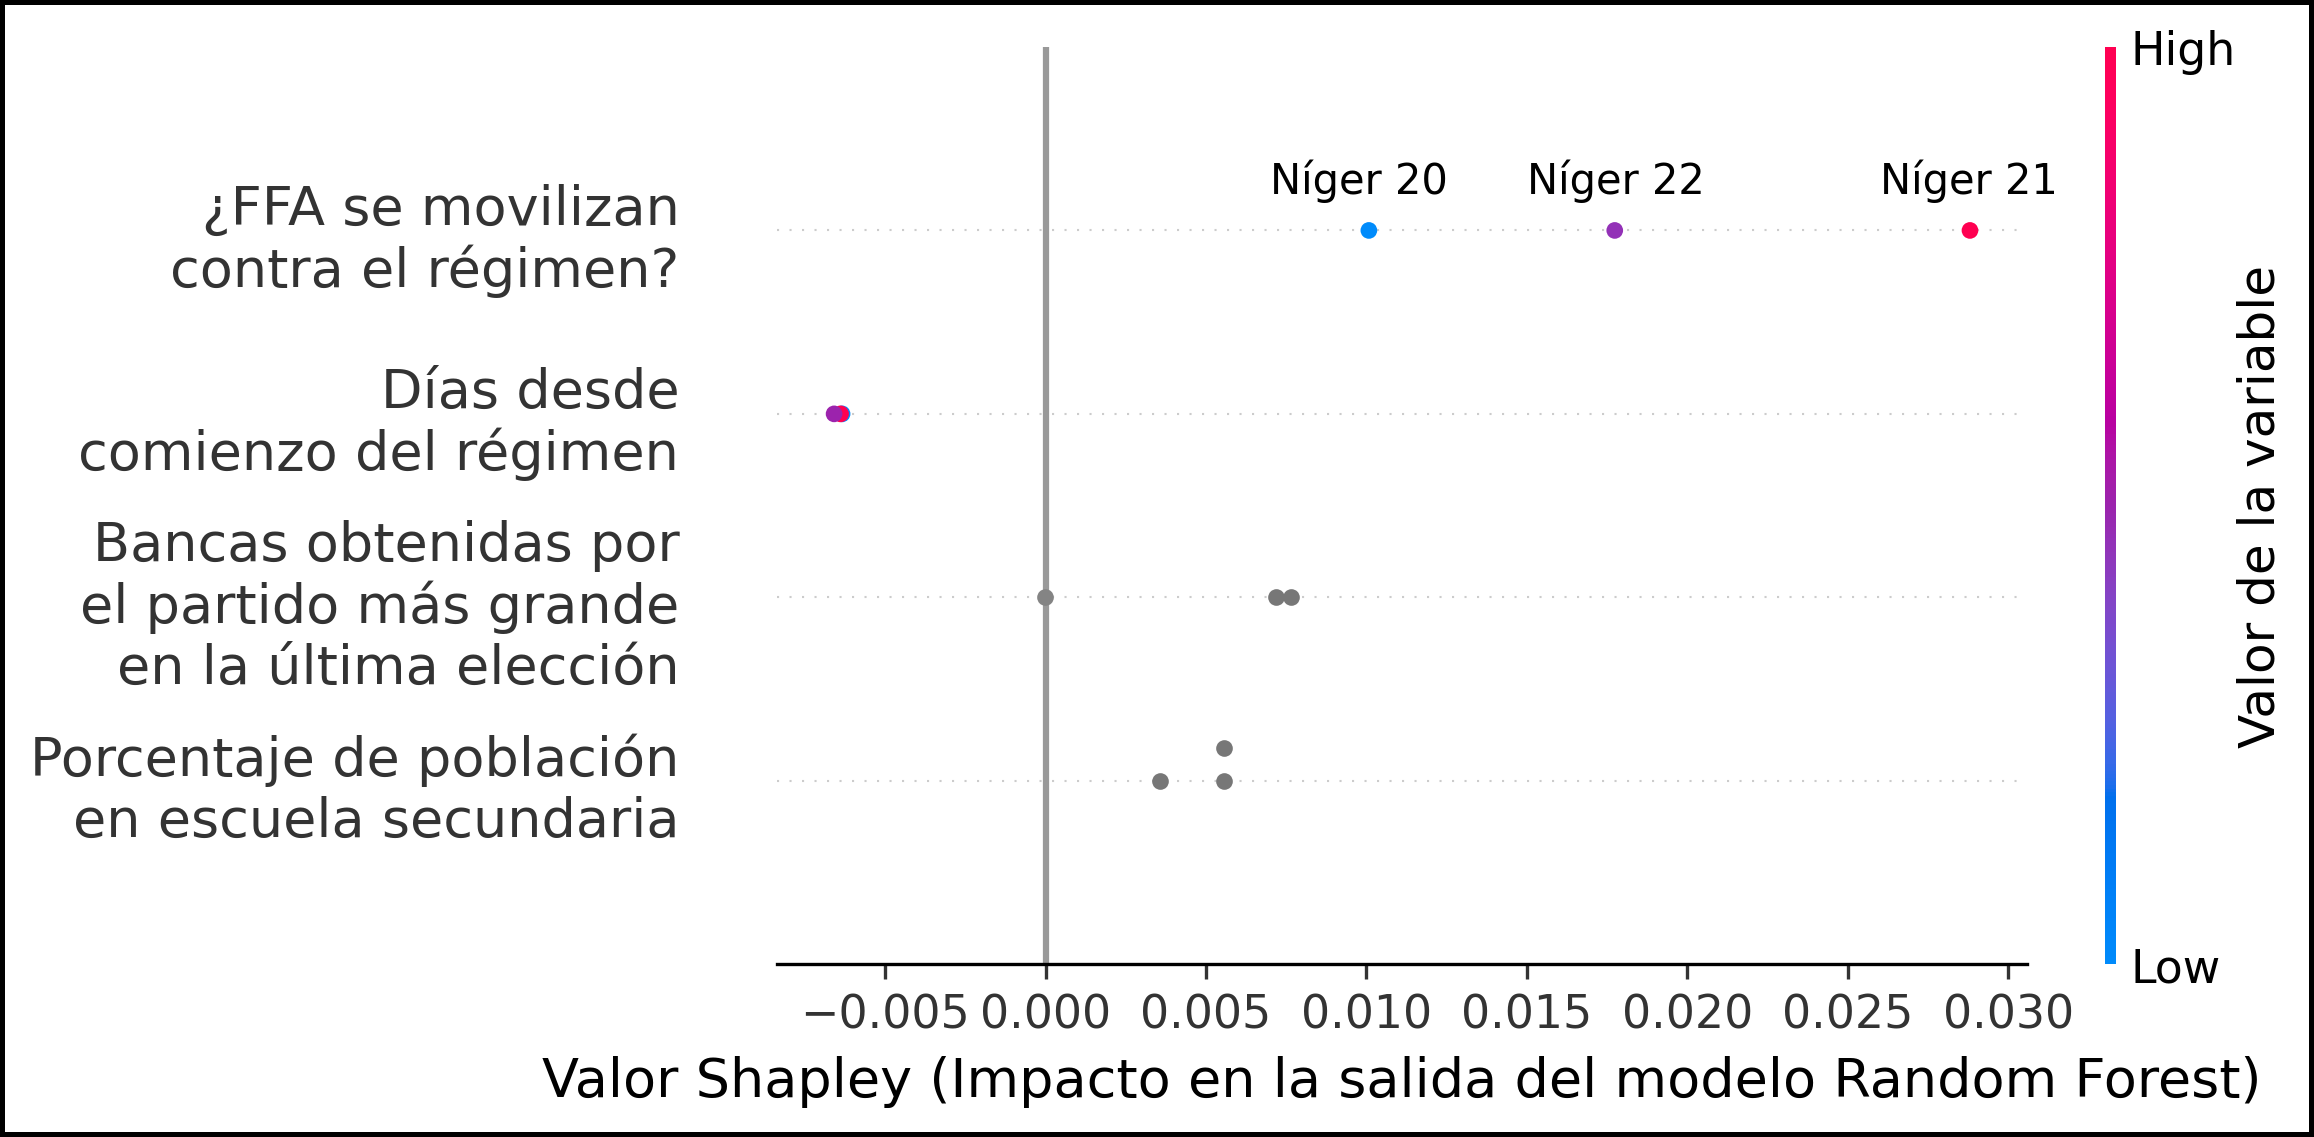
\includegraphics[width=.75\textwidth]{11_shapley_values_rf_niger.png}
 \caption{Shapley values para predicción Níger 2020-2022 (Random Forest)\label{fig:shapley_rf_niger}}
\end{figure}

Lo que se puede aprehender de la figura \ref{fig:shapley_rf_niger} es que en las cuatro variables,
los tres casos (Níger en 2020,2021 y 2023) tienen valores Shapley muy cercanos. Siguiendo esta lógica
se vuelve difícil para el algoritmo predecir si un golpe de Estado sucederá o no.

\begin{figure}[H]
 \centering
 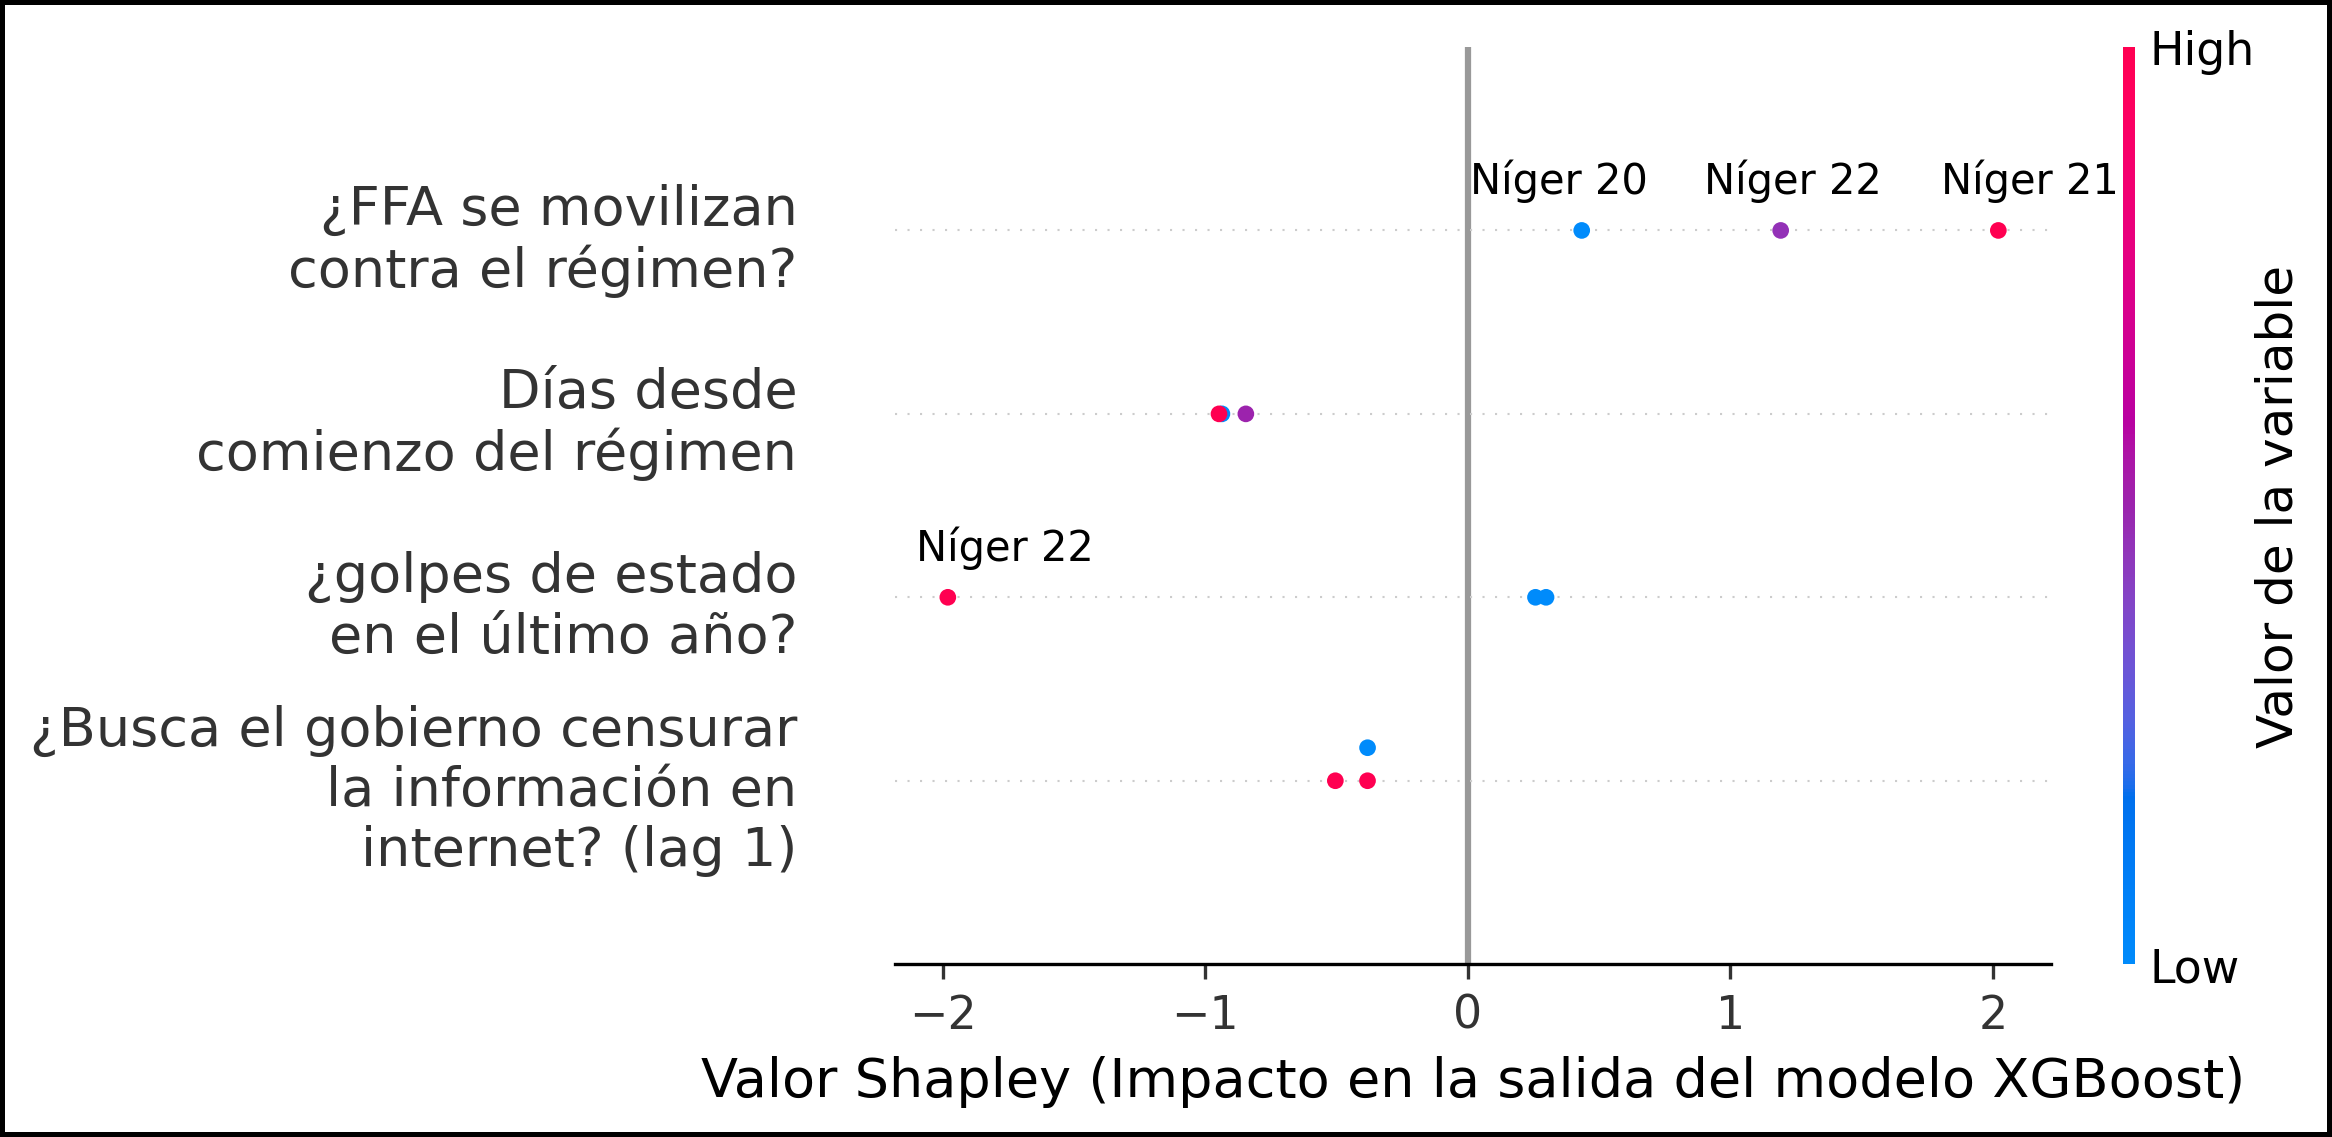
\includegraphics[width=.75\textwidth]{12_shapley_values_xgb_niger.png}
 \caption{Shapley values para predicción Níger 2020-2022 (XGBoost)\label{fig:shapley_xgb_niger}}
\end{figure}

En la figura \ref{fig:shapley_xgb_niger} no parece haber diferencias significativas: en tres de las
cuatro variables los tres casos figuran cercanos y con el mismo signo. Sí resulta interesante que el
lag 1 de la variable objetivo (¿golpes de estado en el último año?) lógicamente separa al caso de
Níger en 2022, pero no parece influir en el resultado final.

El segundo caso que evaluaremos es el de Afganistán en 2021, el cual generó discrepancias entre los
datos y la variable objetivo, si bien uno de los modelos logró predecirlo bien.

\begin{figure}[H]
 \centering
 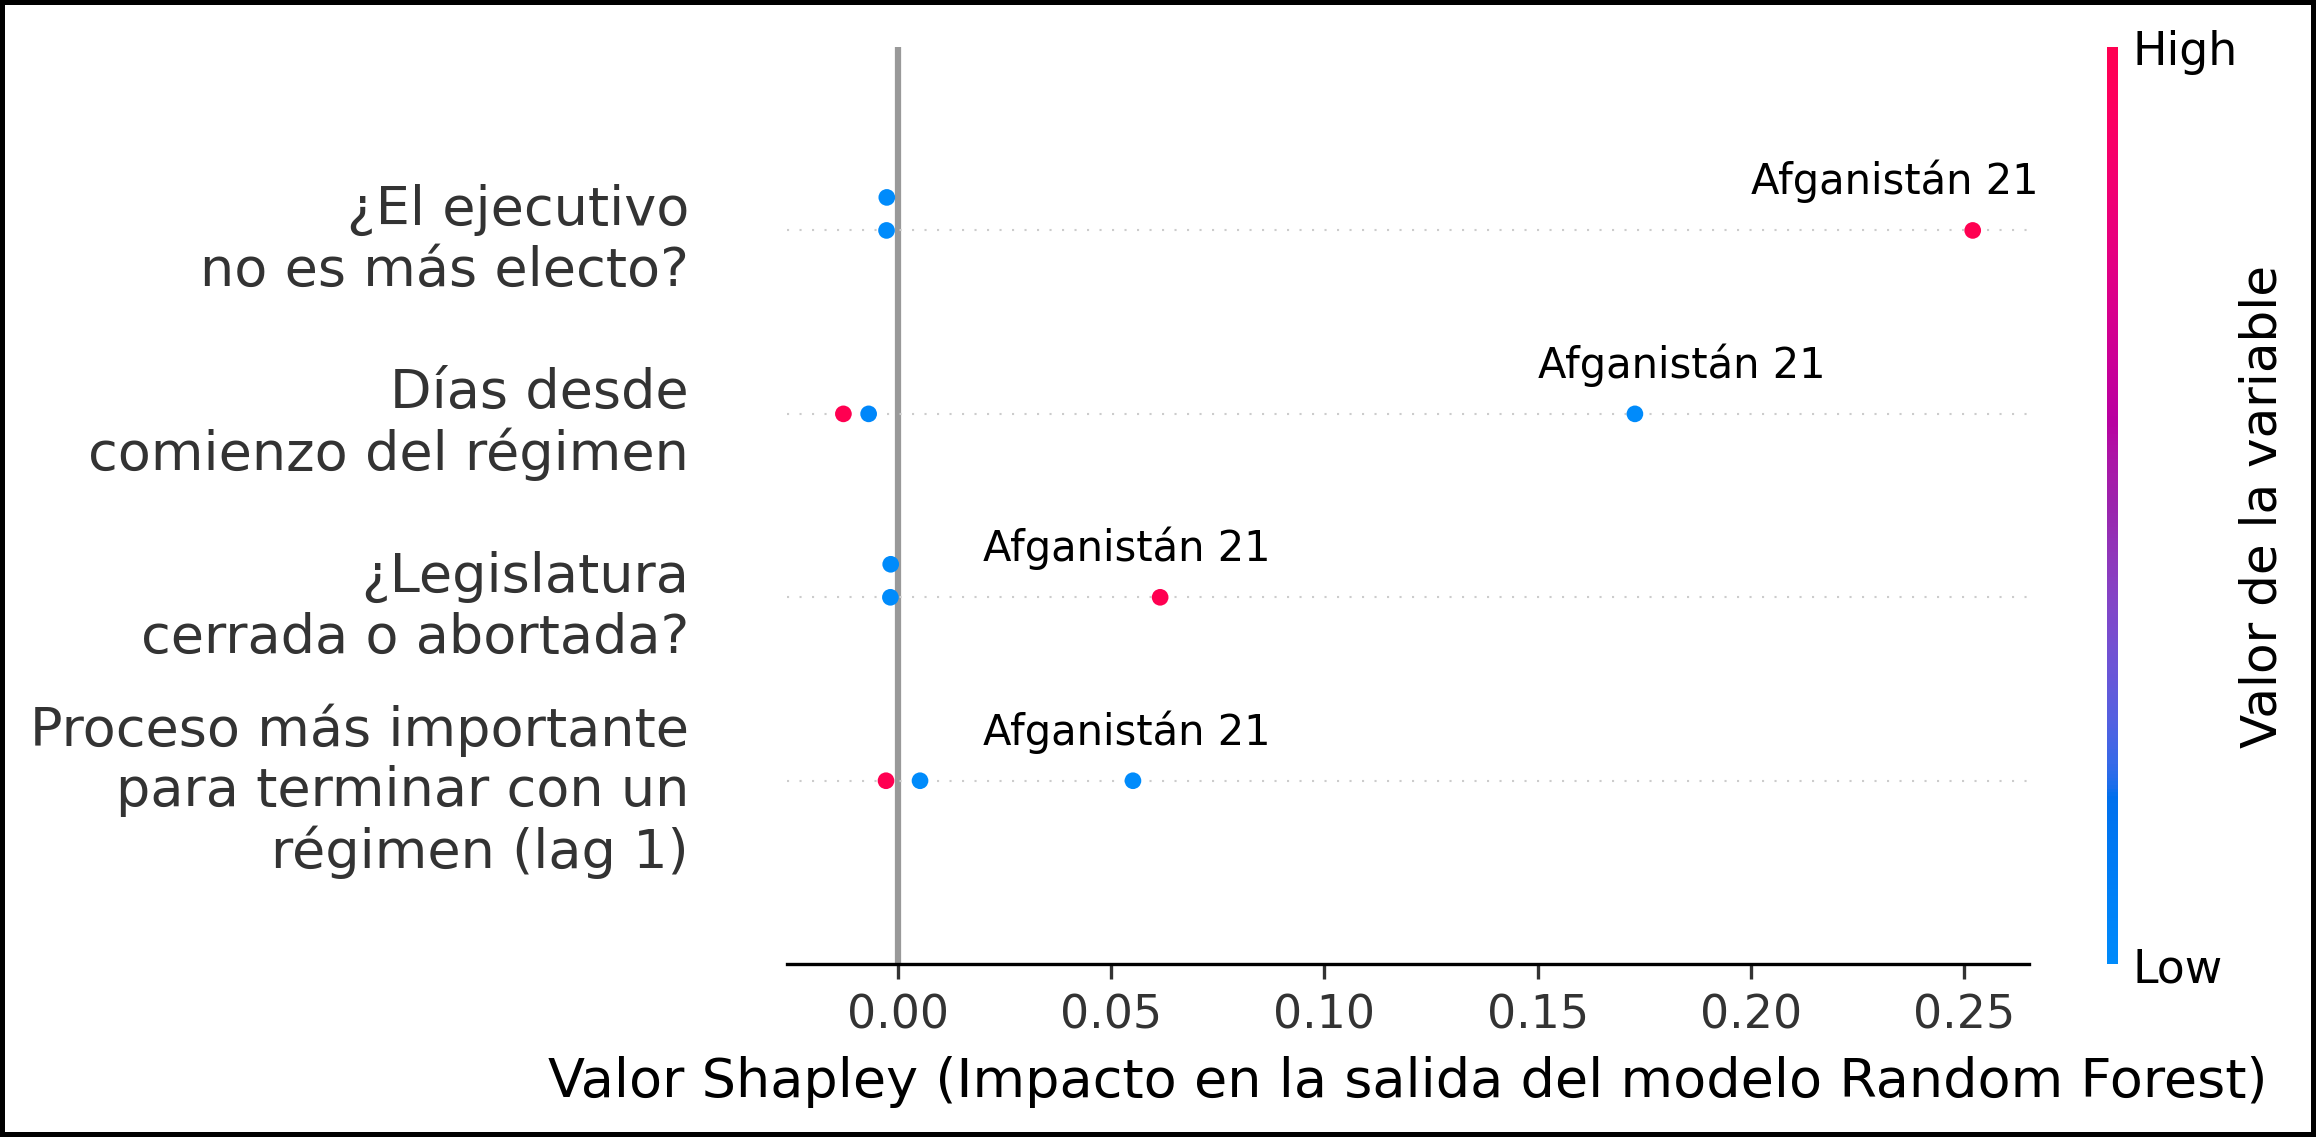
\includegraphics[width=.75\textwidth]{13_shapley_values_rf_afganistan.png}
 \caption{Shapley values para predicción Afganistán 2021 (Random Forest)\label{fig:shapley_rf_afganistan}}
\end{figure}

Lo que se observa con claridad en la figura \ref{fig:shapley_rf_afganistan} es que la cuatro variables
separaron sensiblemente el caso de Afganistán en 2021 del resto de los años. Esto llevó a Random Forest
a predecir incorrectamente este año como uno en el que se generó un golpe.

\begin{figure}[H]
 \centering
 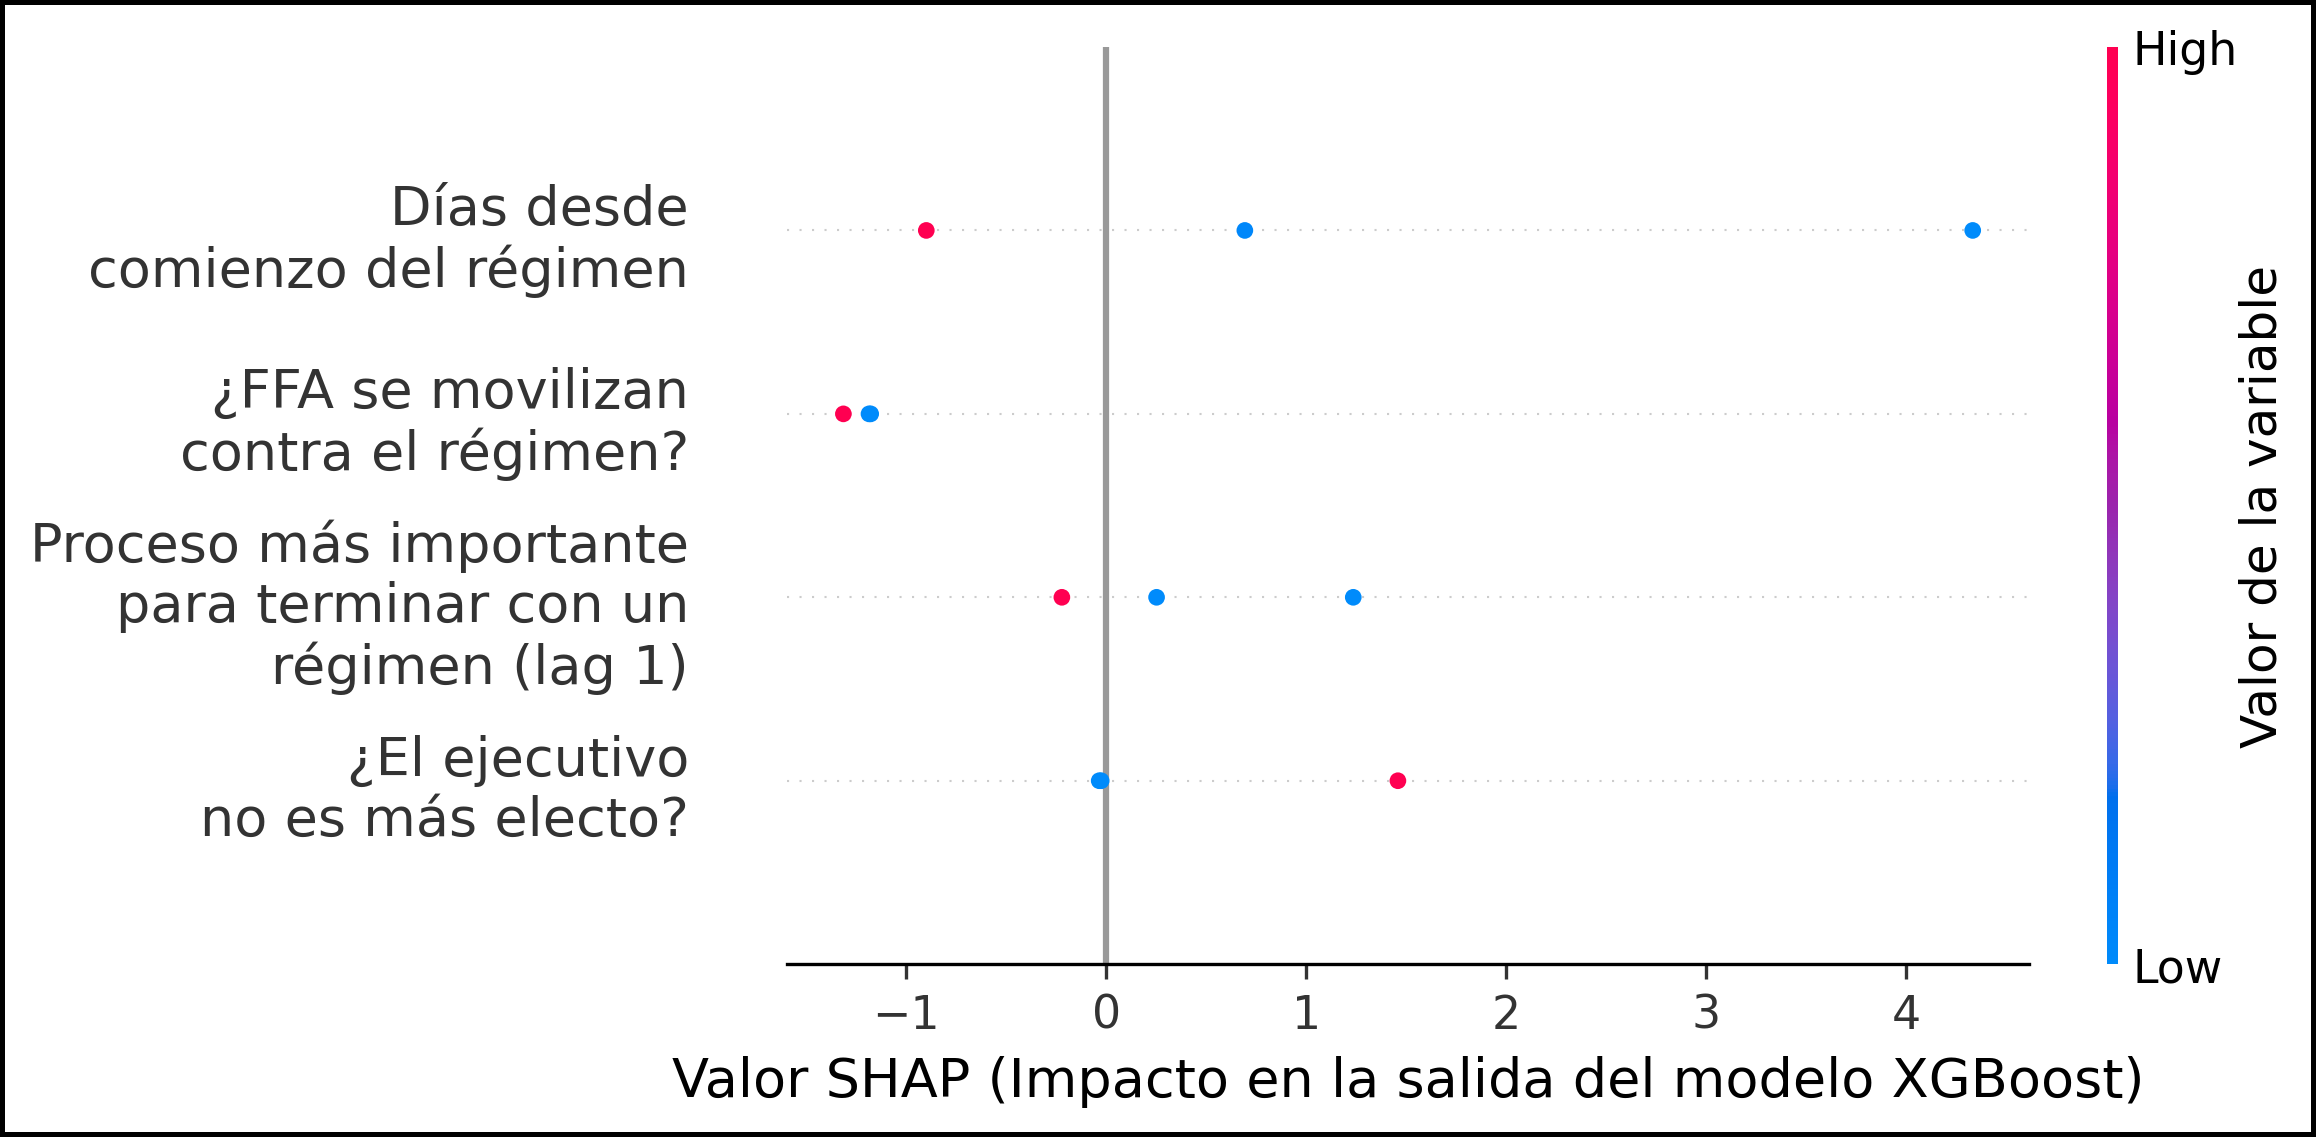
\includegraphics[width=.75\textwidth]{14_shapley_values_xgb_afganistan.png}
 \caption{Shapley values para predicción Afganistán 2021 (XGBoost)\label{fig:shapley_xgb_afganistan}}
\end{figure}

El caso de la figura \ref{fig:shapley_xgb_afganistan} presenta mayores sutilezas. Si bien también
los días desde el comienzo del régimen separa al año 2021 del resto, las últimas dos variables 
presentan a los tres casos mucho más cercanos. Además, la variable que evalúa si las FFAA se movilizan
contra el régimen muestra tres valores muy parecidos (lo cual lo hace incluso imperceptible para la
visualización).

Como conclusión de esta sección, podemos aseverar que ambos algoritmos logran un piso de performance 
apreciable para poder predecir la presencia de golpes de estado en un país y año en particular. Sin 
embargo, XGBoost demostró una mayor capacidad para predecir casos complejos, en los que (como se 
demostró observando la variable del cuadro \ref{tab:shap_rf_regend}) los expertos de V-Dem parecen no 
llegar a un acuredo con Powell y Thyne. De todas formas, ambos algoritmos tienen grandes dificultades 
para predecir golpes 
de estado que no fueron exitosos. Probablemente se deba a que le dan relevancia a atributos que 
describen no sólo un golpe de estado, sino que también un cambio de régimen. El atributo que más 
sobresale es la cantidad de días desde que comenzó el régimen, el cual permite evidenciar la idea 
anterior. Estos algoritmos también recurrieron a variables que describen la interacción entre las 
fuerzas armadas y el poder ejecutivo, así como variables asociadas a la educación política en las 
escuelas.

En la siguiente sección, compararemos las métricas de ambos modelos con los del artículo
de Cebotari et al (\citeyear{Ceb24}) para el FMI; así como las valores Shapley de las variables 
relevantes en ambos casos. También expondremos las limitaciones de este trabajo, tanto en los
datos trabajados como en la metodología utilizada para replicar el trabajo del FMI. Por último,
vincularemos las variables destacadas por los algoritmos con los enfoques expuestos en el marco
teórico.

\section{Discusiones}

En esta sección pondremos a dialogar los resultados de este trabajo de diversas maneras. En primer
lugar, en línea con el objetivo principal del trabajo, compararemos las métricas de los modelos
con los expuestos en el artículo del FMI por Cebotari et al (\citeyear{Ceb24}). Luego, expondremos
las variables importantes de los algoritmos a la luz del marco teórico y el estado del arte. Finalmente,
analizaremos las limitaciones de este trabajo y propondremos recomendaciones para futuros trabajos.


\subsection{Comparación con el artículo del FMI}

Como fue expuesto en las secciones anteriores, el primer objetivo de este trabajo evaluar la performance
de los modelos entrenados con los datos de la fundación Varieties of Democracy en comparación con el modelo
entrenado en el artículo de Cebotari et al para el FMI con alrededor de 10 fuentes de información. Si bien
en el apartado metodológico, Cebotari et al (\citeyear{Ceb24}) describen que algoritmos utilizan, en qué periodo
de tiempo y qué hiperparámetros fueron optimizados; no muestran cuál fue el algoritmo ganador qué se utilizó
para el análisis de resultados. A continuación, mostraremos las principales métricas de performance que
expone el trabajo de Cebotari et al.

\begin{figure}[H]
 \centering
 \fbox{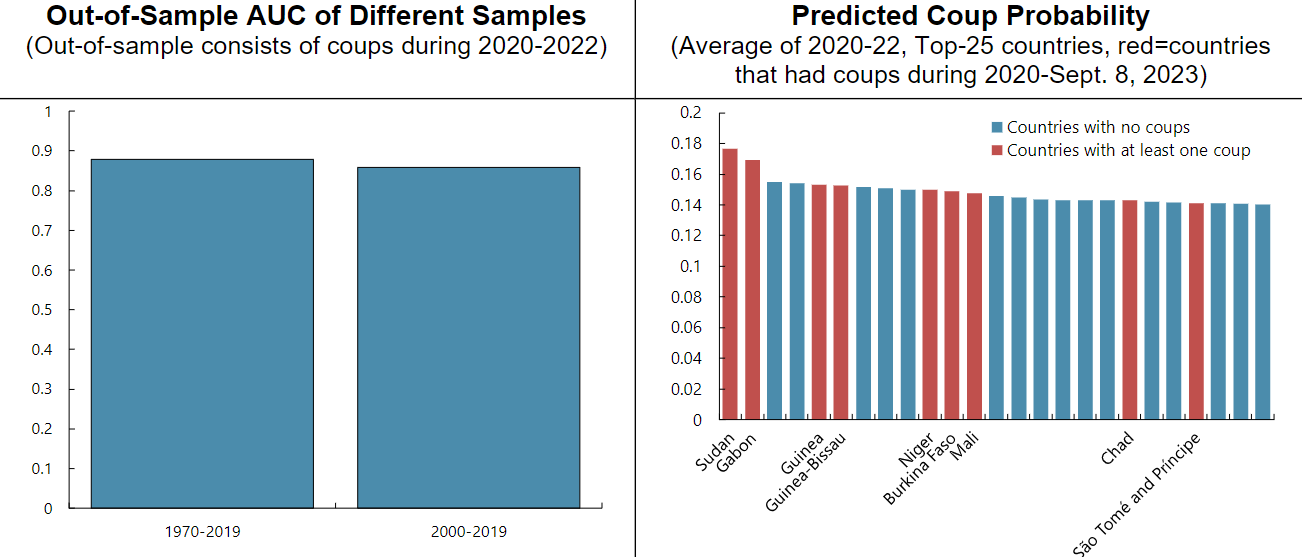
\includegraphics[width=1\textwidth]{15_metricas_cebotari.png}}
 \caption{Performance del modelo FMI (\cite{Ceb24}) \label{fig:metricas_cebotari}}
\end{figure}

La figura \ref{fig:metricas_cebotari} muestra dos visualizaciones: la de la izquierda muestra el área
bajo la curva del modelo entrenado con dos conjuntos de entrenamiento, con datos de entre 1970 a 2019
y otro solo con datos de entre 2000 a 2010. La figura de la derecha, en cambio muestra la probabilidad
promedio de cada país entre 2020 y 2022, marcando en rojo los países que efectivamente sufrieron un
golpe de Estado en alguno de esos años. Con respecto a la métrica del área bajo la curva ROC (AUC), el 
modelo de Cebotari obtuvo alrededor de 0,88 para el conjunto de entrenamiento entre 1970 y 2019. En
cambio el modelo Random Forest y XGBoost obtuvieron ambos un AUC de alrededor 0,75. Para poder comparar
la figura de la derecha replicaremos el análisis en ambos algoritmos.

\begin{figure}[htbp]
 \centering
 \begin{subfigure}[b]{0.49\textwidth}
  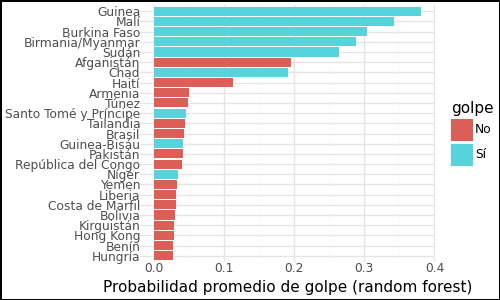
\includegraphics[width=\textwidth]{16_prob_rf_comp.png}
  \caption{Random Forest \label{fig:prob_rf}}
 \end{subfigure}
 \hfill
 \begin{subfigure}[b]{0.49\textwidth}
  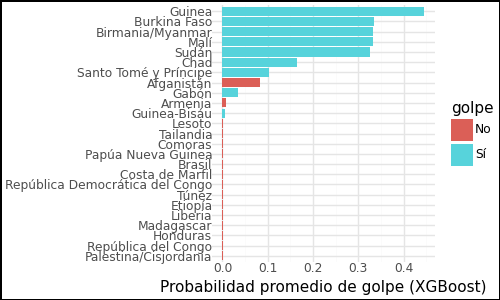
\includegraphics[width=\textwidth]{17_prob_xgb_comp.png}
  \caption{XGBoost \label{fig:prob_xgb}}
 \end{subfigure}
 \caption{Probabilidad promedio de golpe de Estado por país (Random Forest y XGBoost) \label{fig:roc_comp}}
\end{figure}

El modelo del FMI logra incluir en ese top 25 a todos los Estados en donde hubo un golpe
entre 2020 y 2023, con la sola excepción de Birmania/Myanmar. Además, la probabilidad asignada para 
todos estos casos va disminuyendo de manera suave, a tal punto de que la posición 1 tiene una 
probabilidad de casi 0,18 mientras que la posición 25 tiene una probabilidad de alrededor de 0,15. Con
respecto a nuestro algoritmo Random Forest, este si logra incluir en el top 17 a todos los países que 
sufrieron un golpe entre 2020 y 2022, si bien falla en incluir el golpe futuro de Gabón en 2023, así como
los tres golpes de Estado fallidos de Guinea-Bisáu, Níger y Santo Tomé y Príncipe. No es 
el caso de XGBoost, quien no solo logra incluir a Gabón, sino que justo después de ese caso la 
probabilidad de asignar a ese país un golpe de Estado se desploma a casi cero. En definitiva, si bien 
el artículo de Cebotari et al no explicita los verdaderos positivos y falsos positivos; podemos inferir
que lo que genera que su algoritmo alcance valores tan altos es que logra predecir correctamente a los 
golpes de Estado fallidos.

A continuación, observaremos los valores Shapley que obtuvieron las variables más importantes en el
modelo de Cebotari et al (\citeyear{Ceb24}) en la figura \ref{fig:shapley_cebotari} \footnote{Valores 
cercanos al amarillo indican un bajo valor de la variable, mientras que valores cercanos al verde
indican un valor alto.}. Como resulta lógico, en esta visualización figuran algunas variables que son 
ajenas al ámbito político institucional, como
la proporción de adultos mayores (\textit{Share of elder Population}), el crecimiento real del PBI
(\textit{Real GDP growth}) o los ingresos per cápita (\textit{Income per capita}). Sin embargo, también
figuran variables equivalentes a las que observamos en nuestros algoritmos. Por ejemplo, la variable
Años desde el último golpe (\textit{Years since last coup}) es equivalente a la variable que mide la
cantidad de días desde el comienzo del régimen, el cual figura entre las dos variables con valores Shapley
más altos en la figura \ref{fig:shapley_rf} y \ref{fig:shapley_xgb}. Con una relación menos directa, también podemos
mencionar el grado de democratización (\textit{Degree of Democratization}), el gasto militar (\textit{Military
Expenditure}) y la cantidad de golpes anteriores (\textit{Number of Coups Before}); los cuales guardan 
similitud con variables de la base de datos V-Dem. Incluso podrían generarse estas variables en futuros 
trabajos en la etapa de ingeniería de atributos.

\begin{figure}[H]
 \centering
 \fbox{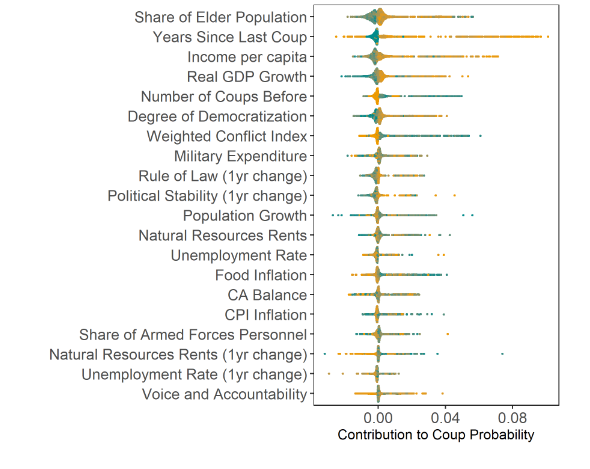
\includegraphics[width=.75\textwidth]{18_shapley_values_cebotari.png}}
 \caption{Shapley values para modelo FMI (\cite{Ceb24}) \label{fig:shapley_cebotari}}
\end{figure}

Como conclusión general de esta sección, el algoritmo generado por Cebotari et al demuestra una mayor 
performance a la hora de predecir golpes de Estado en un año y país en particular. En especial, goza
de mayor poder de predicción para los intentos fallidos. Se puede inferir que esta mayor capacidad
predictiva surge del amplio abanico de atributos con los que cuenta su base de datos, que provienen de
diversas fuentes externas y que describen fenómenos políticos, económicos, sociales y poblacionales. De
todas formas, no es banal destacar que el hecho de que el trabajo del FMI haya incluido tantas fuentes
externas hace más probable que existan serias difiultades para replicar el trabajo en años futuros. En 
cambio, en nuestro trabajo nos cercioramos de excluir del entrenamiento atributos ajenos a la encuesta
desarrollada todos los años por la fundación Varieties of Democracy. De esa manera, tenemos mayor 
confianza de poder replicar este trabajo en el futuro en la medida de que la encuesta y la fundación 
que la respalda continúen realizando su trabajo.

\subsection{Análisis teórico de los resultados}

En esta sección haremos una breve reflexión teórica sobre las variables destacadas por los tres 
algoritmos (XGboost, Random Forest y el presentado por Cebotari et al (\citeyear{Ceb24})). En primer lugar
podemos destacar la variable que indica los días desde el comienzo del régimen, el cual figura tanto en 
XGBoost como en Random Forest como uno de los principales atributos a considerar para sus predicciones.
Como contraparte también figura en XGBoost y en el algoritmo del FMI la presencia de golpes en años
anteriores. Lo que se puede rescatar de estos atributos es que una democracia que logra perdurar en el
tiempo ininterrumpidamente se vuelve cada vez menos propensa a sufrir interrupciones institucionales en
forma de golpe de Estado.

Otro tipo de variables se relacionan de manera más obvia con la variable objetivo, como la interrupción de
la legislatura o que el poder ejecutivo no sea más electo. De todas formas, esto le imprime un sesgo
democrático a los algoritmos, en el sentido de que esperan que los golpes de Estado se 
realizen contra democracias y no contra dictaduras. De forma no tan directa, el algoritmo XGBoost nos hace
llamar la atención sobre la declaración de un estado de emergencia, el cual augura una fuerte
inestabilidad política en el país que es declarada.

Adicionalmente, destacan las variables asociadas al poder relativo de las fuerzas armadas sobre el gobierno,
así como por su nivel de movilización contra el gobierno. El algoritmo del FMI también agrega el porcentaje
de personal militar por sobre la población y el gasto militar del Estado. Sin ser una novedad, esta 
información coloca a las fuerzas armadas como actores ineludibles en cualquier interrupción del orden 
constitucional

Otro punto de interés es la presencia de variables asociadas a la educación primaria y secundaria, así como
de la presencia de enseñanza sobre valores políticos. Este tipo de atributos respaldan los postulados de
Lipset (\citeyear{lipset1959some}). Siguiendo su línea de pensamiento, un fortalecimiento de la enseñanza
de valores políticos en la población asegura el fortalecimiento de la legitimidad de un régimen democrático,
uno de los dos pilares junto con la eficacia para que una democracia se mantenga en el tiempo.

Como último aporte, no quisieramos dejar de mencionar la presencia del crecimiento real del PBI en el
algoritmo desarrollado por Cebotari et al (\citeyear{Ceb24}), fundamentalmente porque contradice las teorías
esbozadas por Hungington (\citeyear{huntington68political}) de
que el acelerado crecimiento económico genera inestabilidad política.

En síntesis, los algoritmos entrenados en este trabajo no tienden a dialogar de manera directa con los
postulados de los autores citados en el marco teórico. Esto sucede fundamentalmente porque los datos de
la base de datos utilizadas son inherentes al ámbito político institucional, mientras que los teóricos
sociales buscan explicaciones más amplias y multicausales, que involucren procesos no solo políticos sino
también económicos, sociales y culturales.

\subsection{Limitaciones}

En esta sección mostraremos las limitaciones que ha encontrado este trabajo para lograr el objetivo de
reproducir e artículo de Cebotari et al (\citeyear{Ceb24}) y lograr un algoritmo que prediga igual o mejor
en términos del área bajo la curva ROC. En primer lugar, a la hora de optimizar hiperparámetros, el artículo
no indica en qué rangos de hiperparámetros se manejaron; lo cual implicó que se haya tenido que trabajar
con rangos amplios de los mismos, volviéndolo más costoso computacionalmente. Esto generó problemas
particularmente con Random Forest, ya que es un algoritmo que suele tardar varios minutos en entrenarse 
dependiendo del valor de los hiperparámetros que se optimizaron en el artículo.

En segundo lugar, fue recurrente la incapacidad de ambos algoritmos para predecir golpes de Estado fallidos.
Esto parece ser indicador de que los datos de V-Dem no logran dar suficientes señales de que un golpe intentó
perpretarse infructuosamente en un momento determinado.

Después, la capacidad computacional limitada con la que se podía disponer impidió que se pudiera explorar
la utilización de todas las variables del conjunto de datos, puesto que se quitaron algunas versiones de las 
mismas variables para incorporar sus variantes lag (especulando con que tendrían mayor valor para la predicción
). Por último, si bien no se condice con el objetivo de reproducir el artículo del FMI, el conjunto de
datos de V-Dem cuenta con información anterior a 1970, la cual de haberse utilizado podría haber
generado algoritmos con mayor capacidad predictiva.

\section{Conclusiones}
En este trabajo se buscó reproducir hallazgos del artículo de Cebotari et al (\citeyear{Ceb24})
para el Fondo Monetario Internacional, utilizando los mismos algoritmos (Random Forest y XGBoost), optimizando
los mismos hiperparámetros y utilizando la misma variable objetivo (golpes de Estado en un país y año en
particular, según la base de datos de Powell y Thyne (\citeyear{Pow11})). La diferencia de este trabajo radicó
en utilizar otro conjunto de datos para entrenar los algoritmos, de manera de evaluar el poder predictivo
sobre golpes de Estados de variables exclusivamente políticas e institucionales.

Con respecto a los resultados obtenidos, ambos algoritmos lograron un piso de performance de
alrededor del 0,75 por ciento del área bajo la curva ROC. XGBoost logró imponerse sobre Random Forest apenas
por predecir correctamente como negativo el caso de Afganitán en 2021 (cuadro \ref{tab:resultados}). 
Este caso en particular, por el valor de las variables más destacadas por Random Forest, figura como 
un caso particularmente conflictivo entre
los expertos que construyeron los datos de V-Dem para ese año, quienes dieron muchas señales para 
categorizar ese año como uno en donde sucedió un golpe de Estado, y la variable objetivo construida con los 
datos de Powell y Thyne que indican lo contrario. De todas formas, algo común en ambos algoritmos fue la 
incapacidad de predecir golpes de Estado fallidos ocurridos durante la serie del conjunto de 
testeo (2020-2022). Este hallazgo nos hace cuestionar la calidad de los datos para predecir este subtipo de 
hechos políticos.

Luego, se evaluaron los valores Shapley de ambos algoritmos (figuras \ref{fig:shapley_rf} y 
\ref{fig:shapley_xgb}), en donde se destacaron las variables asociadas
a la duración del régimen, al poder relativo de las fuerzas armadas frente al poder ejecutivo, el nivel
educativo de la población y la formación política incluida, así como la declaración de estados de emergencia.
Para profundizar el análisis de los valores Shapley, tomamos dos casos particulares: Níger en 2021, el cual
ambos algoritmos fallaron en predecirlo como golpe de Estado; y Afganistán en el mismo año, en donde solo XGBoost
logró predecirlo correctamente. En el caso de Níger, al visualizar los valores Shapley se observa con
claridad como los dos algoritmos fallan en separar el caso de este país en 2021 de los otros dos años
(figuras \ref{fig:shapley_rf_niger} y \ref{fig:shapley_xgb_niger}). Con
respecto a Afganistán, se observa cómo Random Forest separa fuertemente la situación de este país en 2021
con respecto al mismo país en 2020 y 2021 (figura \ref{fig:shapley_rf_afganistan}); mientras XGBoost, si 
bien cuenta también con valores Shapley que separan este caso del resto, se apoya en otras variables 
importantes para el algoritmo que acercan lo suficiente los tres años del país para predecirlo 
correctamente como caso negativo (figura \ref{fig:shapley_xgb_afganistan}).

Acto seguido, pusimos a dialogar los resultados con los del artículo de Cebotari et al. Si bien el artículo
no muestra con claridad el valor de la métrica de performance ni de las probabilidades asignadas a cada caso,
las figuras del artículo (figura \ref{fig:metricas_cebotari}) muestran con claridad que el área bajo la curva
de su algoritmo figura apenas por debajo del 90 por ciento del área bajo la curva, por encima de los
valores obtenidos por los algoritmos de este trabajo. De estos resultados inferimos que el algoritmo del 
artículo para el FMI tiene una mayor capacidad de predecir intentos de golpes de Estado fallidos. También
evaluamos brevemente los valores Shapley del algoritmo de Cebotari (figura \ref{fig:shapley_cebotari}), 
encontrando similitudes entre las variables destacadas por ambos trabajos, si bien logicamente destaca 
variables exógenas al ámbito político y más asociadas a la economía y la demografía.

Finalmente, se esbozó un intento de vinculación de los resultados con los postulados expuestos en el marco
teórico. El principal inconveniente de esta sección fue que los autores traidos a la discusión intentaron
generar teorías que incluyen variables que exceden el ámbito político, como la economía,
la demografía o el capital humano. De todas formas, se encontraron vasos comunicantes entre las variables
importantes de Random Forest asociadas a la eduación (figuras \ref{fig:feat_imp_rf} y \ref{fig:shapley_rf})
con la teoría de la modernización expuesta con Lipset (\citeyear{lipset1959some}).

El hecho de haber realizado un trabajo acotado a la metodología utilizada por un artículo anterior
nos limitó en lo que respecta al entrenamiento de los algoritmos y la optimización
de hiperparámetros, así como es probable que haya restringido la capacidad de predicción, puesto que el 
conjunto de datos de V-Dem cuenta con muchos más años que los utilizados en 
el trabajo del FMI. De todas formas, estas limitaciones nos presentan muchas posibilidades para trabajos 
futuros, puesto que implica modificar distintos aspectos 
metodológicos, ya sea para mejorar la performance predictiva de los modelos como para ganar capacidad
explicativa. En primer lugar, se pueden incorporar otro tipo de algoritmos. Un ejemplo es LightGBM, un 
algoritmo de boosting que es el principal competidor a XGBoost para ganar poder predictivo. También es 
posible buscar buenas predicciones con algoritmos menos complejos, como la regresión logística, que además 
permite explicar de manera mucho más precisa las variables que influyen en la predicción con la sola 
utilización de sus parámetros.

Adicionalmente, se puede ampliar la optimización de hiperparámetros. En este trabajo solo se optimizaron
un par en cada algoritmo, cuando se podría intentar optimizar todos. XGBoost en particular cuenta con alrededor
de 20 hiperparámetros que se podrían utilizar. Además, al utilizar una optimización bayesiana con una cantidad
de iteraciones fija, la cantidad de tiempo invertido no crecería tanto puesto que el algoritmo se encargaría
de maximizar el área bajo la curva lo antes posible en esa cantidad de iteraciones.

Otra línea de investigación implica mejorar la cantidad y calidad de datos. El conjunto de datos de V-Dem
cuenta con información de calidad sobre todo el siglo xx hasta la actualidad, incluyendo incluso variables
histórica hasta 1789. Eso, sumado a la incorporación de otras versiones de las variables (promedios,
desvíos estándar, entre otros) darían más poder de predicción a los algoritmos. Alternativamente, se podría
diseñar un problema de clasificación múltiple, que sortee el problema que encontraron los algoritmos para 
predecir golpes fallidos. De esa manera se podría codificar como 0 si no sucedió un golpe, como 1 si fue un
golpe fallido y como 2 si fue un golpe exitoso.

Por último, si bien intentamos predecir golpes de Estado, el enfoque del trabajo impide generar
predicciones para el futuro; por lo que nos focalizamos en generar explicaciones sobre golpes en el
pasado reciente. Si quisieramos predecir golpes para el año actual, deberíamos contar con 
una enorme cantidad de variables que toman tiempo en codificarse y que se suelen publicar hacia el final del
año. Por ese motivo, se podría rediseñar la variable objetivo, adelantando una n cantidad de años la columna
objetivo, para que cuando se evalúa el modelo en el conjunto de testeo, en realidad se esté prediciendo
si sucederá un golpe en cierta cantidad de años. De esa manera se le podría dar un uso práctico a los
algoritmos además de uno meramente académico.

En definitiva, y más allá de las limitaciones encontradas, podemos considerar que el trabajo tuvo un resultado
satisfactorio. Si bien, no alcanzó el nivel predictivo del artículo de Cebotari et al, si tuvo una performance
muy buena para predecir golpes de Estado exitosos. Además, gracias a los valores Shapley pudimos detectar
rapidamente qué valores intervinieron en la generación de predicciones, lo cual
gana especial relevancia dado que trabajamos con un conjunto de datos de miles de atributos que pueden
ser difíciles de destacar para evaluar el nivel democrático o la estabilidad institucional en un análisis
descriptivo tradicional.

\section{Anexo}
\subsection{Código}
La totalidad del código así como este documento en formato latex y PDF se encuentran en un repositorio abierto 
de Github de José Saint Germain (\href{https://github.com/josesg998/esp_data_mining}{Acceso al 
repositorio}). En el mismo se describe la secuencia de códigos a correr para la obtención de 
datos, la ingeniería de atributos, la optimización bayesiana, la corrida final, el análisis 
exploratorio de datos y el análisis de resultados de los algoritmos.

\subsection{Gráficos y cuadros adicionales}
\begin{figure}[H]
 \centering 
 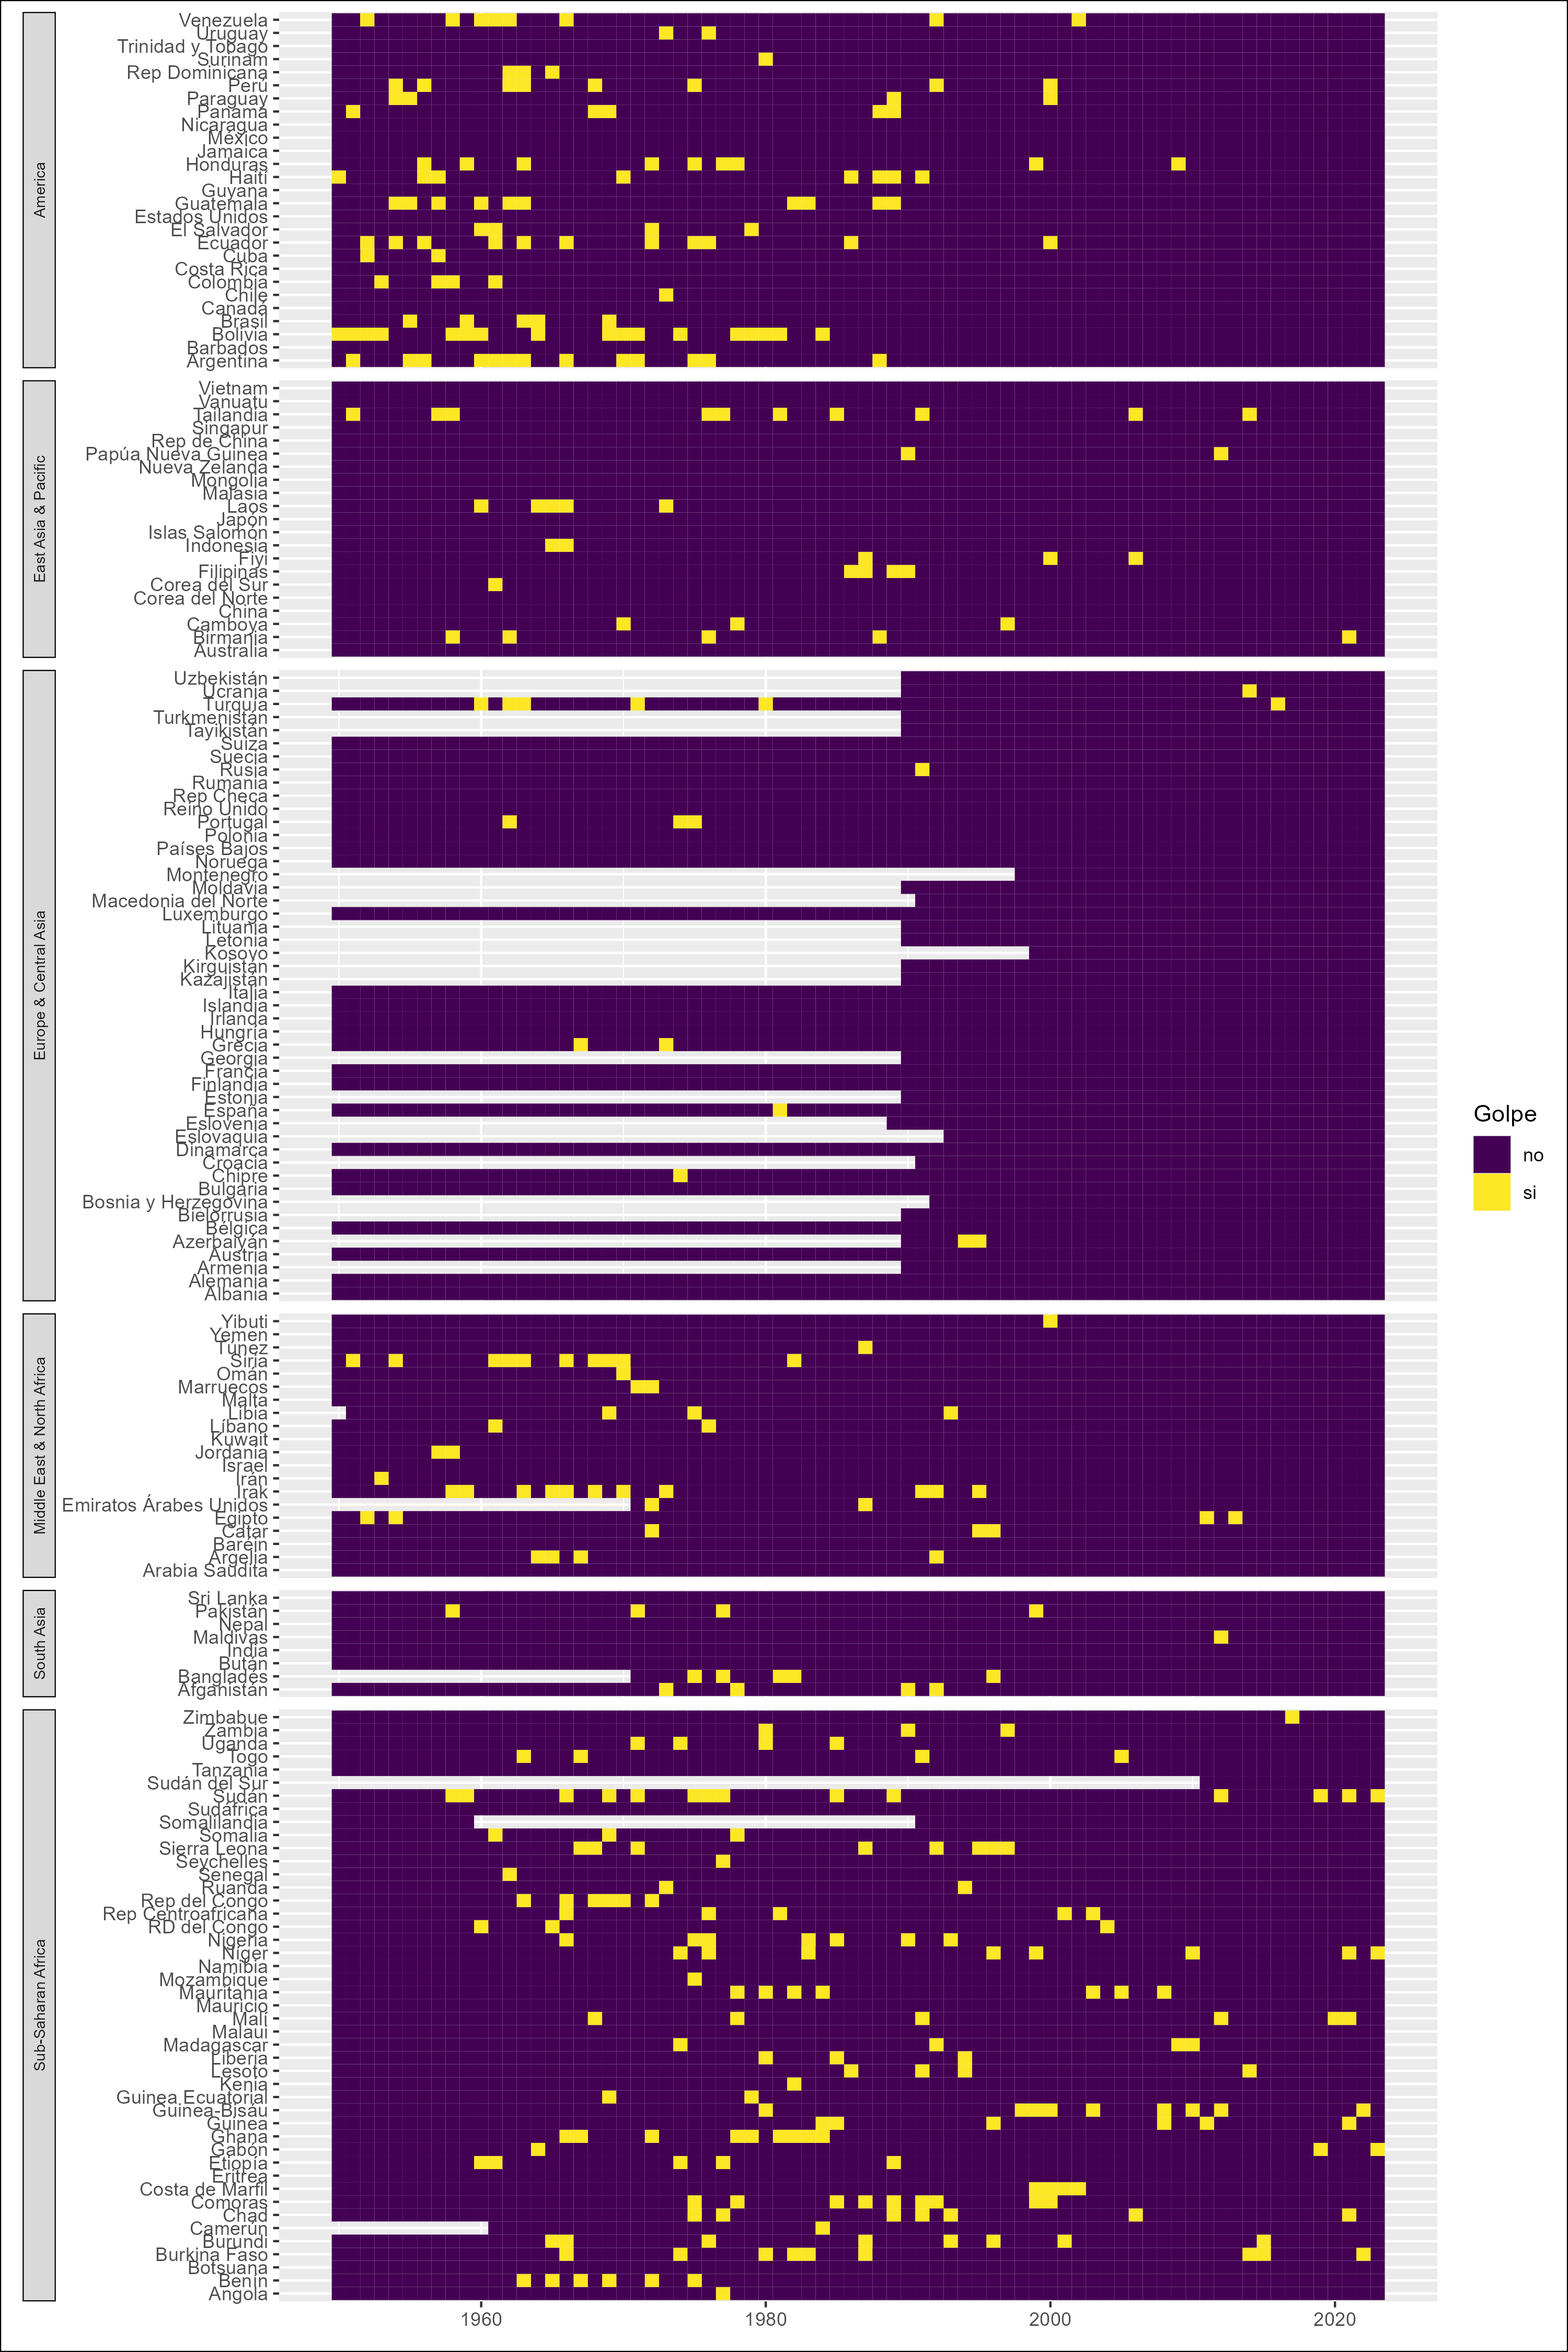
\includegraphics[width=1\textwidth]{4_golpes_anios.png}
 \caption{Conteo de golpes por año y región (\cite{Pow11})\label{fig:golpes_anios}}
\end{figure}

\begin{table}[H]
 \begin{tabular}{ll}
  \toprule
  Variable & Descripción \\
  \midrule
  v2regdur & Días desde comienzo del régimen \\
  v2regendtypems\_0\_lag\_1 & ¿El régimen terminó por un golpe de estado? (lag 1) \\
  v2x\_hosinter & ¿El ejecutivo no es más electo? \\
  v2xlg\_leginter & ¿Legislatura cerrada o abortada? \\
  v2regendtype\_lag\_1 & Proceso más importante para terminar con un régimen (lag 1) \\
  v2x\_ex\_military & Influencia de las FFAA sobre el Poder Ejecutivo \\
  v2regoppgroupsact\_5 & ¿FFA se movilizan contra el régimen? \\
  coup\_lag\_1 & ¿golpes de estado en el último año? \\
  v2x\_ex\_military\_lag\_1 & Influencia de las FFAA sobre el Poder Ejecutivo (lag 1) \\
  v2expathhs & ¿Cómo llega el jefe de estado al gob? \\
  v2regendtype\_lag\_5 & ¿Qué proceso fue el más importante en el fin del régimen? (lag 5) \\
  v2clpolcl\_lag\_1 & Libertad para todos los grupos políticos \\
  v2csanmvch\_2\_lag\_10 & Grupos antisistema que mezclan métodos legales e ilegales (lag 10) \\
  v2juhcind & Decisiones importantes de la Corte Suprema alineadas con el gobierno \\
  v2exfxtmhs\_lag\_1 & Duración máxima del mandato del jefe de Estado (lag 1) \\
  v2edpoledprim\_lag\_5 & ¿Se enseña en la primaria contenidos con valores políticos? (lag 5) \\
  v2elpeace & Violencia durante período electoral \\
  v2pesecsch & Porcentaje de población en escuela secundaria \\
  v2lgqugent & Cuota femenina en la cámara baja (o cámara única) \\
  v2ellostlg & Bancas obtenidas por el partido más grande en la última elección \\
  v2casoe\_1 & Emergencia nacional: no declarada pero medidas preparatorias tomadas \\
  v2casoe\_4 & Declaración de estado de emergencia nacional por conflicto armado \\
  v2casoe\_6 & Declaración de estado de emergencia nacional por otros motivos \\
  v2exagehos\_lag\_5 & Año de nacimiento del jefe de estado (lag 5) \\
  v2elvotbuy\_lag\_1 & ¿Hubo evidencia de compra de votos en la última elección? (lag 1) \\
  v2asuffrage & Porcentaje de adultos con derecho a votar mayores que la edad mínima \\
  v2mecenefi\_lag\_1 & ¿Busca el gobierno censurar la información en internet? (lag 1) \\
  \bottomrule
  \end{tabular}
 \caption{Nombre original de variables y su descripción \label{tab:vars}}
\end{table}

\printbibliography

\end{document}